\documentclass[8pt, oneside]{beamer}   	% use "amsart" instead of "article" for AMSLaTeX format
\usepackage{geometry}                		% See geometry.pdf to learn the layout options. There are lots.
%\geometry{letterpaper}                   		% ... or a4paper or a5paper or ... 
%\geometry{landscape}                		% Activate for rotated page geometry
%\usepackage[parfill]{parskip}    		% Activate to begin paragraphs with an empty line rather than an indent
\usepackage{graphicx}				% Use pdf, png, jpg, or eps§ with pdflatex; use eps in DVI mode
								% TeX will automatically convert eps --> pdf in pdflatex		
\usepackage{amssymb}
\usepackage{amsmath}
\usepackage{textpos} % package for the positioning
\usepackage{eso-pic}


\usepackage {tikz}
\usetikzlibrary {positioning}
\definecolor {processblue}{cmyk}{0.96,0,0,0}

%SetFonts

%SetFonts
\newcommand{\supp}{\operatorname{supp}}
\newcommand{\dist}{\operatorname{dist}}
\newcommand{\divr}{\operatorname{div}}
\newcommand{\tdiv}{\operatorname{div}}
\newcommand{\ess}{\operatorname{ess}}
\newcommand{\rotore}{\operatorname{rot}}
\newcommand{\curl}{\operatorname{\textbf{curl}}}
\newcommand{\bcurl}{\operatorname{\textbf{curl}}}
\newcommand{\tr}{\operatorname{tr}}
\newcommand{\bA}{\textbf{A}}
\newcommand{\ba}{\textbf{a}}
\newcommand{\bb}{\textbf{b}}
\newcommand{\bB}{\textbf{B}}
\newcommand{\bc}{\textbf{c}}
\newcommand{\bC}{\textbf{C}}
\newcommand{\bd}{\textbf{d}}
\newcommand{\bD}{\textbf{D}}
\newcommand{\be}{\textbf{e}}
\newcommand{\bE}{\textbf{E}}
\newcommand{\bff}{\textbf{f}}
\newcommand{\bF}{\textbf{F}}
\newcommand{\bg}{\textbf{g}}
\newcommand{\bG}{\textbf{G}}
\newcommand{\bi}{\textbf{i}}
\newcommand{\bI}{\textbf{I}}
\newcommand{\bj}{\textbf{j}}
\newcommand{\bJ}{\textbf{J}}
\newcommand{\bh}{\textbf{h}}
\newcommand{\bH}{\textbf{H}}
\newcommand{\bk}{\textbf{k}}
\newcommand{\bK}{\textbf{K}}
\newcommand{\bl}{\textbf{l}}
\newcommand{\bL}{\textbf{L}}
\newcommand{\bm}{\textbf{m}}
\newcommand{\bM}{\textbf{M}}
\newcommand{\bn}{\textbf{n}}
\newcommand{\bN}{\textbf{N}}
\newcommand{\bp}{\textbf{p}}
\newcommand{\bP}{\textbf{P}}
\newcommand{\bo}{\textbf{o}}
\newcommand{\bq}{\textbf{q}}
\newcommand{\bQ}{\textbf{Q}}
\newcommand{\br}{\textbf{r}}
\newcommand{\bR}{\textbf{R}}
\newcommand{\bs}{\textbf{s}}
\newcommand{\bS}{\textbf{S}}
\newcommand{\btau}{\boldsymbol{\tau}}
\newcommand{\bt}{\textbf{t}}
\newcommand{\bv}{\textbf{v}}
\newcommand{\bV}{\textbf{V}}
\newcommand{\bw}{\textbf{w}}
\newcommand{\bW}{\textbf{W}}
\newcommand{\bu}{\textbf{u}}
\newcommand{\bU}{\textbf{U}}
\newcommand{\by}{\textbf{y}}
\newcommand{\bY}{\textbf{Y}}
\newcommand{\bbx}{\textbf{x}}
\newcommand{\bX}{\textbf{X}}
\newcommand{\blambda}{\boldsymbol{\lambda}}
\newcommand{\beps}{\boldsymbol{\varepsilon}}
\newcommand{\bphi}{\boldsymbol{\phi}}
\newcommand{\bPhi}{\boldsymbol{\Phi}}
\newcommand{\bpsi}{\boldsymbol{\psi}}
\newcommand{\bomega}{\boldsymbol{\omega}}
\newcommand{\bsigma}{\boldsymbol{\sigma}}
\newcommand{\bSigma}{\boldsymbol{\Sigma}}
\newcommand{\bxi}{\boldsymbol{\xi}}
\newcommand{\aaa}{\`a}
\newcommand{\eee}{\`e}
\newcommand{\iii}{\`i}
\newcommand{\ooo}{\`o}
\newcommand{\uuu}{\`u}
\newcommand{\aaaa}{\'a}
\newcommand{\eeee}{\'e}
\newcommand{\iiii}{\'i}
\newcommand{\oooo}{\'o}
\newcommand{\uuuu}{\'u}
\newcommand{\AAA}{\`A}
\newcommand{\EEE}{\`E}
\newcommand{\III}{\`I}
\newcommand{\OOO}{\`O}
\newcommand{\UUU}{\`U}
\newcommand{\AAAA}{\'A}
\newcommand{\EEEE}{\'E}
\newcommand{\IIII}{\'I}
\newcommand{\OOOO}{\'O}
\newcommand{\UUUU}{\'U}
\newcommand{\ND}{\mathcal{ND}}
\newcommand{\RT}{\mathcal{RT}}

%%% norm and abs
\newcommand\norm[1]{\left\lVert#1\right\rVert}
\newcommand\abs[1]{\left\vert#1\right\vert}


\usepackage[utf8]{inputenc}
\usetheme{PaloAlto}
\definecolor{Colorrr}{rgb}{1, 0.88, 0.5}
\usecolortheme[named=Colorrr]{structure}
%\logo{
\includegraphics[width=1.16cm,height=1.16cm]{img/logo_ics2}\vspace{1pt}\hspace{-10000pt}}

\newcommand\AtPagemyUpperLeft[1]{\AtPageLowerLeft{%
\put(\LenToUnit{0.81\paperwidth},\LenToUnit{0.881\paperheight}){#1}}}
\AddToShipoutPictureFG{
  \AtPagemyUpperLeft{{
\includegraphics[width=2.5cm,keepaspectratio]{img/logo_ics}}}
}%



\setbeamercolor{frametitle}{fg=black}

\usepackage{color}
% Colors
%------------------------------------------------------------------------------------------------------------------------------------------
\definecolor{bgblue}{rgb}{0.04,0.39,0.53}
\definecolor{dkgreen}{cmyk}{1,0.58,1,0.33}
\definecolor{mygreen}{rgb}{0,0.6,0}
\definecolor{bgorange}{cmyk}{0,0.1,0.7,0}
\definecolor{orange}{cmyk}{0,0.9,0.9,0}
\definecolor{navyblue}{cmyk}{1,0.7,0.36,0.4}
\definecolor{brown}{cmyk}{0.62,0.79,0.93,0.22}
\definecolor{tan}{cmyk}{0.14,0.21,0.47,0}
\definecolor{dkgrey}{cmyk}{0.72,0.7,0.75,0.15}
\definecolor{blueviolet}{rgb}{0.5412    0.1686    0.8863}
\definecolor{gold}{rgb}{0.9    0.6431         0}


\newcommand{\colr}{\color{red}}
\newcommand{\colb}{\color{blue}}
\newcommand{\colg}{\color{mygreen}}
\newcommand{\colo}{\color{orange}}
\newcommand{\colw}{\color{white}}
\newcommand{\colt}{\color{tan}}
\newcommand{\coln}{\color{brown}}
\newcommand{\colk}{\color{black}}
\newcommand{\colc}{\color{cyan}}
\newcommand{\colm}{\color{magenta}}
\newcommand{\coly}{\color{yellow}}
\newcommand{\colp}{\color{blueviolet}}
\newcommand{\colgold}{\color{gold}}

\newcommand{\titlecolor}[1]{\frametitle{\textcolor{dkgrey}{ \textbf{#1}}}}
%------------------------------------------------------------------------------------------------------------------------------------------




%\addtobeamertemplate{frametitle}{}{%
%\begin{textblock*}{100mm}(\textwidth,-0.84cm)
%
\includegraphics[height=1.5cm,width=1.5cm,keepaspectratio]{img/logo}
%\end{textblock*}}
 
%------------------------------------------------------------------------------------------------------------------------------------------

% titlepage definitions
%------------------------------------------------------------------------------------------------------------------------------------------




  
  
  
\title{ \textcolor{dkgrey}{  \textbf{Monotone multilevel for FOSLS linear elastic contact} }}
\author{\textcolor{dkgrey}{\textbf{G. Rovi}, B. Kober, G. Starke, R. Krause}}
\institute{Universit\"at Duisburg\,-\,Essen, Germany \\ Universit\aaa~della Svizzera italiana, Switzerland}



\setbeamertemplate{sidebar right}{}
\setbeamertemplate{footline}{%
\hfill\usebeamertemplate***{navigation symbols}
\hspace{1cm}\insertframenumber{}/\inserttotalframenumber}
\begin{document}
 \begin{frame}
\titlepage
\begin{figure}[htbp!]
	
\includegraphics[scale=0.7]{img/logo_ics}
	\quad
		
\includegraphics[scale=0.3]{img/essenlogo}
\end{figure}
\end{frame}








 



%%%%%%%%%%%%%%%%%%%%%%%%%%%%%%%%%%%%%%%%%%
%%%%%%%%%%%                   SLIDE 1                %%%%%%%%%%%%%%%
%%%%%%%%%%%%%%%%%%%%%%%%%%%%%%%%%%%%%%%%%%
\begin{frame}
\titlecolor{Examples of contact problems}
\begin{figure}[htbp!]
	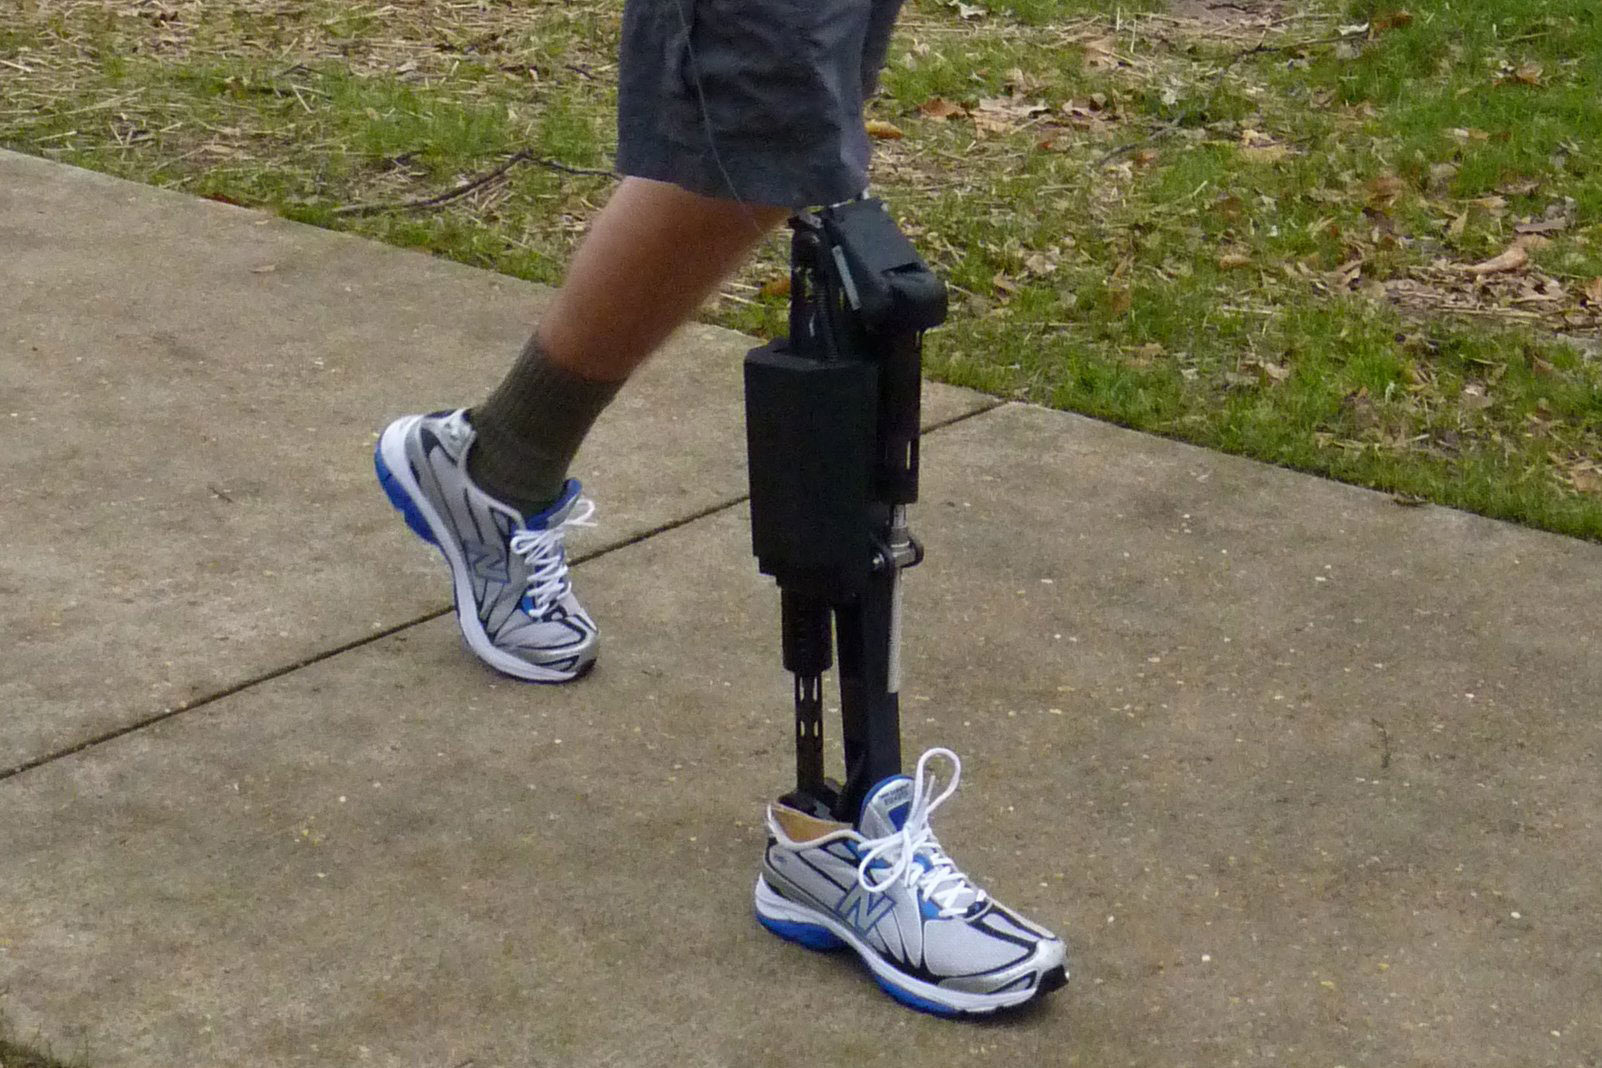
\includegraphics[width=0.35\textwidth]{img/walking}
		\label{abb_arc}\qquad 
			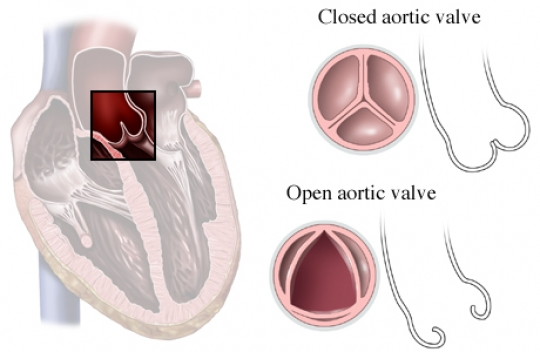
\includegraphics[width=0.35\textwidth]{img/aorticvalve}
		\label{abb_arc}
\end{figure}
\begin{figure}[htbp!]
		\centering
	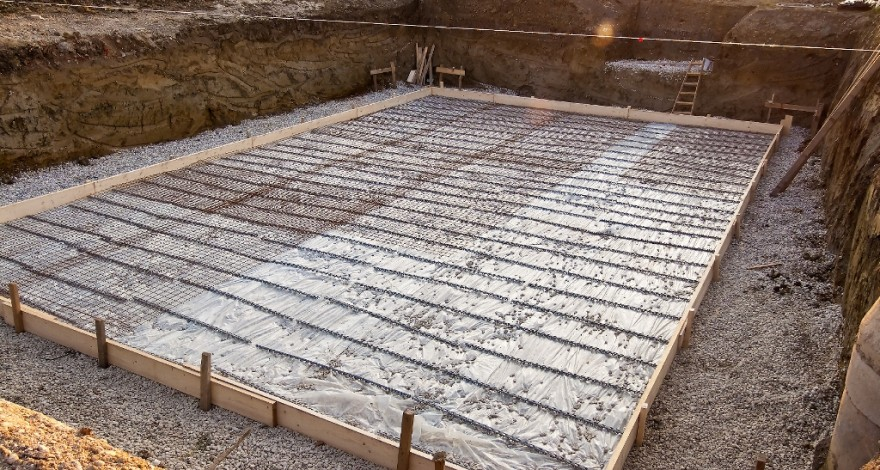
\includegraphics[width=0.4\textwidth]{img/foundation}
		\label{abb_arc}
\end{figure}
\begin{itemize}
\item Contact problems with incompressible materials. 
\item Quantities of interest: the forces generated by the contact.
\end{itemize}
\end{frame}


%%%%%%%%%%%%%%%%%%%%%%%%%%%%%%%%%%%%%%%%%%
%%%%%%%%%%%                   SLIDE 2                %%%%%%%%%%%%%%%
%%%%%%%%%%%%%%%%%%%%%%%%%%%%%%%%%%%%%%%%%%
\begin{frame}
\titlecolor{Signorini's problem: strong formulation}

\begin{itemize}
\item  \textbf{First Order System Linear Elasticity:}
\begin{align*}
\colk
\footnotesize
\begin{cases}
\text{div} \bsigma + \bff=0 & \Omega  \qquad \colk{\text{momentum balance equation}}\\
\mathcal{A} \bsigma - \boldsymbol{\varepsilon}(\bu)=0 &\Omega \qquad \colk{\text{constitutive law}}\\
\colb \bu = \bu_D & \colb \Gamma_D\quad \:\:\: \colk{{\text{Dirichlet BC}}}\\
\colg \bsigma  \bn = \bt_N & \colg \Gamma_N\quad  \:\:\:\colk{{\text{Neumann BC}}}\\
\end{cases} 
\end{align*}
\scriptsize
where  $\boldsymbol{\varepsilon}(\bu)= \dfrac{1}{2} (\nabla \bu+\nabla \bu^T)$, $\boldsymbol{\mathcal{A}}=\dfrac{1}{2 \mu} \left(\bsigma-\dfrac{\lambda}{d \lambda + 2 \mu } \text{tr} \bsigma \bI\right)$ and $\mu$, $\lambda$ are the Lam\eeee  ${}$ parameters
\normalsize
\item { \textbf{Contact Constraints:} }\\
\colk
\small
$ \partial \Omega=\Gamma_C \cup  \Gamma_D \cup  \Gamma_N$, $\Gamma_i \cap  \Gamma_j =\emptyset$ for $i,j=D,N,C, i \neq j$
\end{itemize}
\begin{align*}\colo
\footnotesize
\begin{cases}
\bu \cdot \colgold \bn \colo- \colp{g} \colo  \leq 0 \quad & \Gamma_C  \:\:  \colk{\text{impenetrability}}\\
(\bsigma \colgold \bn \colo) \cdot \colgold \bn \colo \leq 0 \quad & \Gamma_C  \:\:  \colk{\text{direction of the surface pressure}}\\
 \left(\bu \cdot\colgold \bn \colo -\colp{g} \colo \right) \left( (\bsigma\colgold \bn \colo) \cdot \colgold \bn \colo \right) =0 &\Gamma_C  \:\:  \colk{\text{complementarity condition}}\\
\colgold \bt_i^T \colo(\bsigma \colgold \bn \colo) =0  \quad & \Gamma_C  \:\: \colk{\text{frictionless condition}}
\end{cases}
\end{align*}
%\end{flushleft}
\begin{figure}[htbp!]
		\centering
	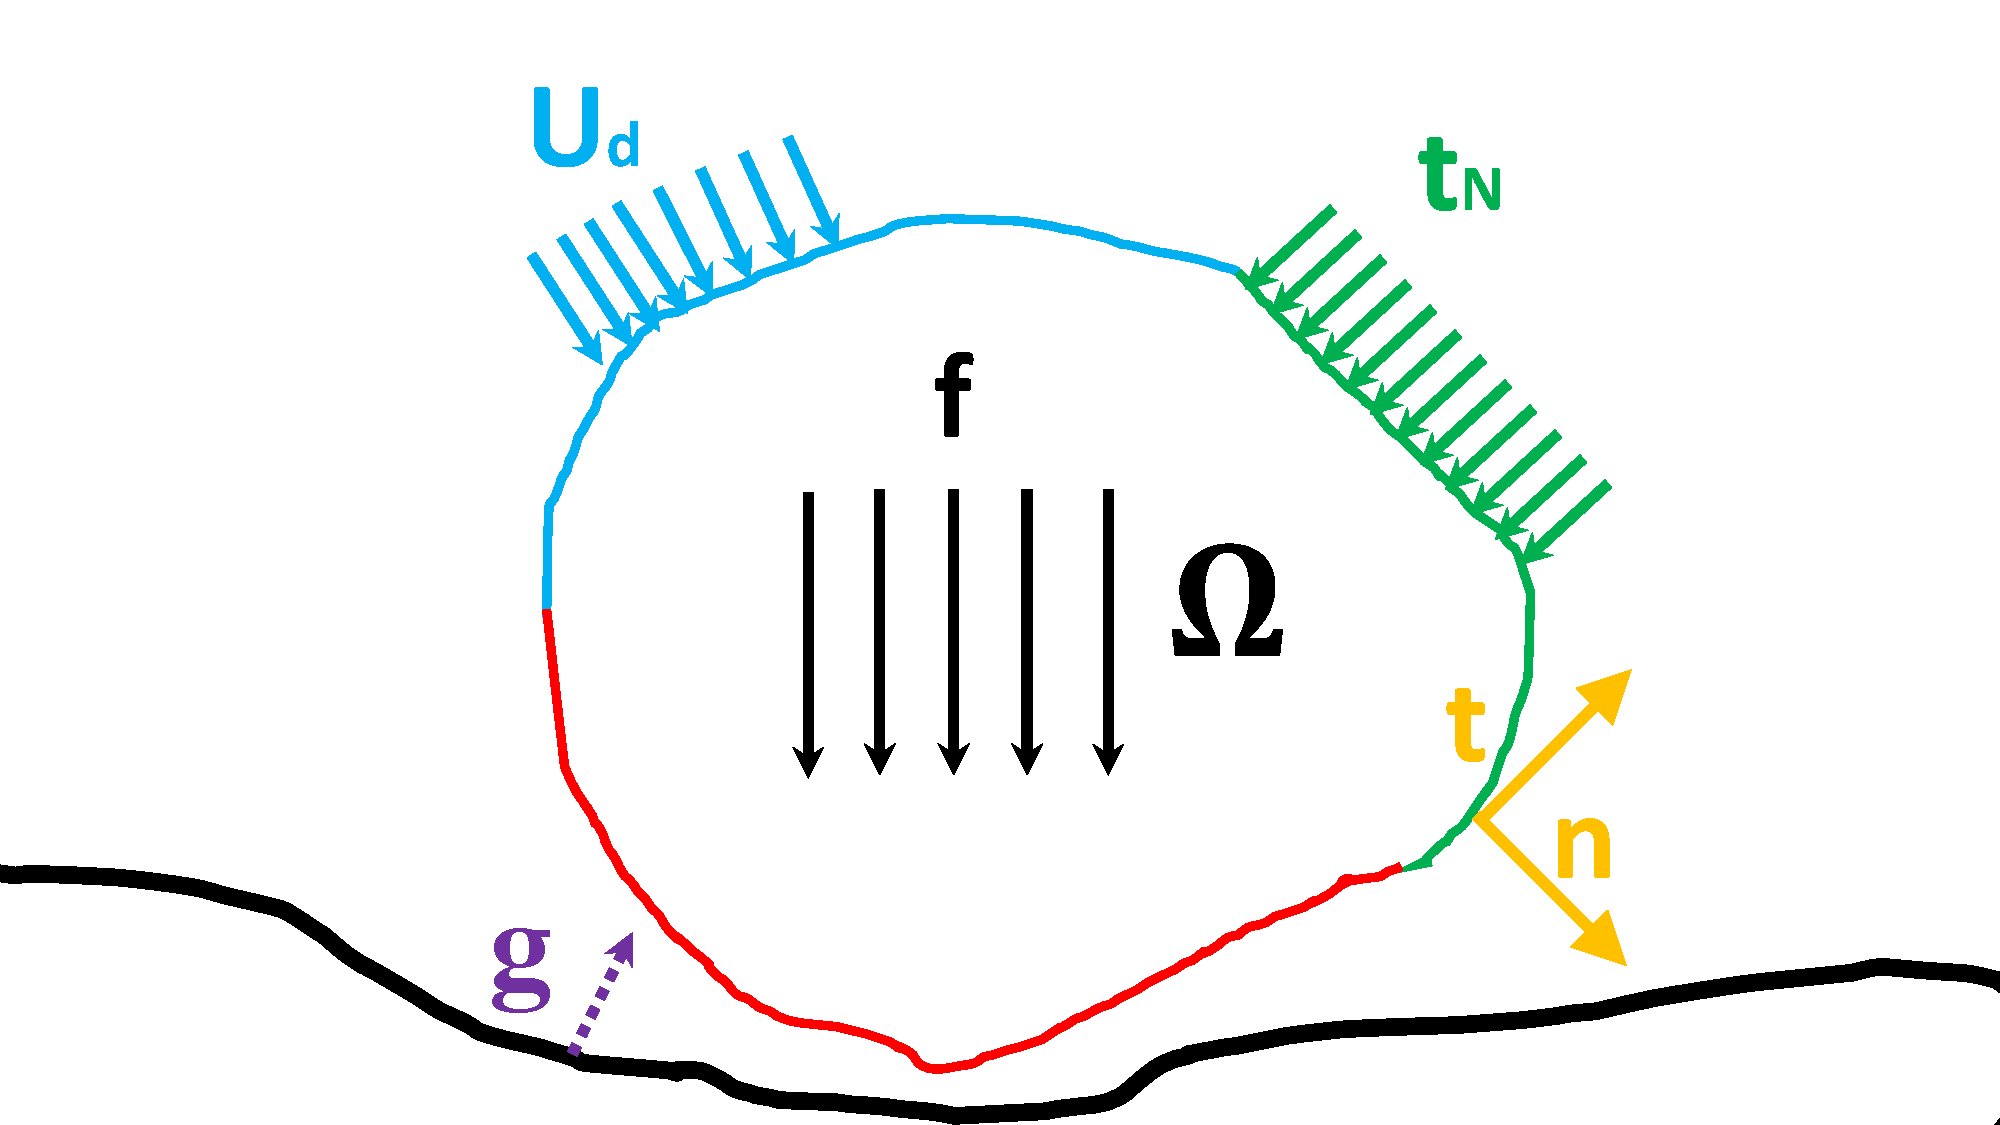
\includegraphics[width=0.35\textwidth]{img/contactproblem.pdf}\qquad
	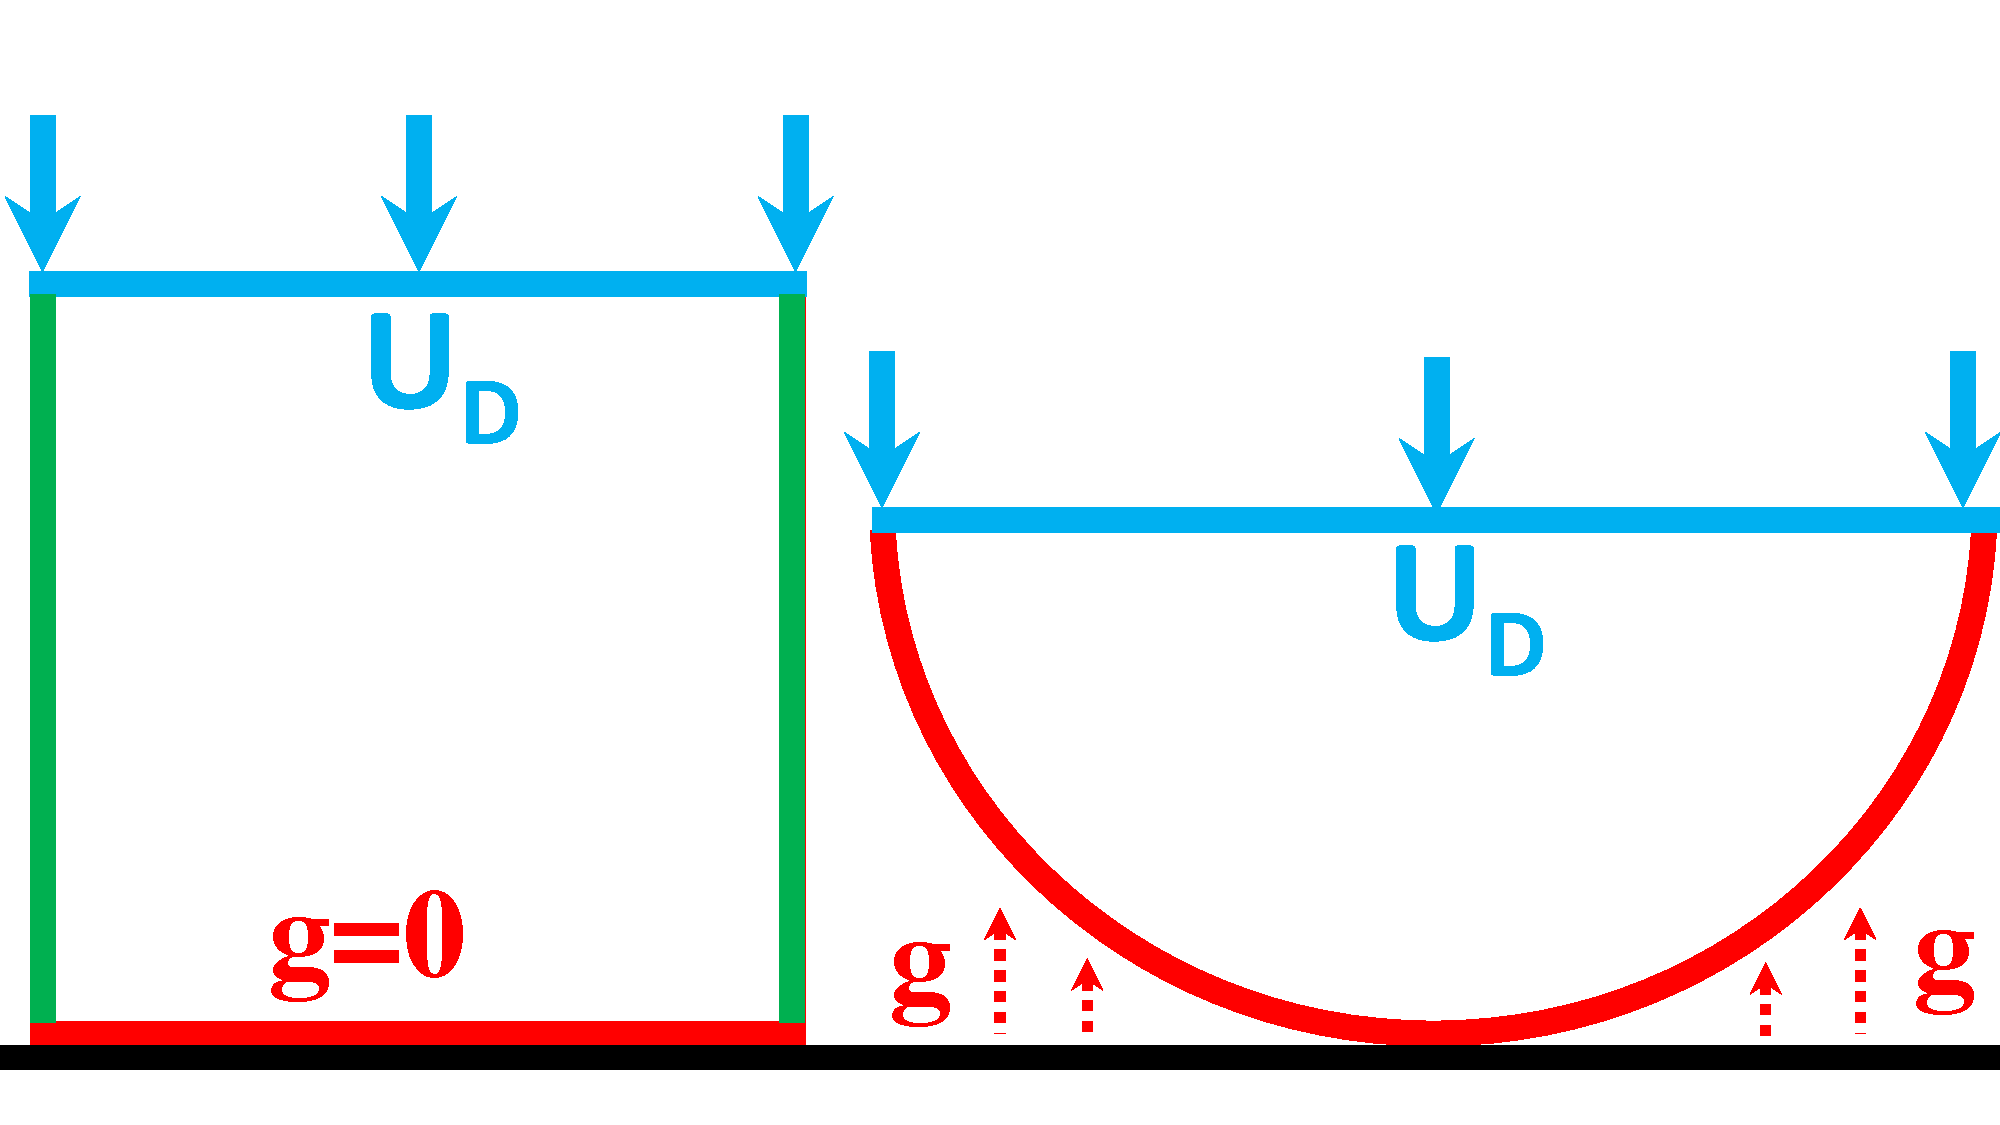
\includegraphics[width=0.35\textwidth]{img/squarecircle.pdf}
		\label{abb_arc}
\end{figure}
%\tiny{Rolf Krause. A nonsmooth multiscale method for solving frictional two-body contact problems in 2d and 3d with multigrid efficiency. SIAM Journal on Scientific Computing, 31(2):1399-1423, 2009.}
\end{frame}


%%%%%%%%%%%%%%%%%%%%%%%%%%%%%%%%%%%%%%%%%%
%%%%%%%%%%%                   SLIDE 3                %%%%%%%%%%%%%%%
%%%%%%%%%%%%%%%%%%%%%%%%%%%%%%%%%%%%%%%%%%

\begin{frame}
\titlecolor{The Least-Squares Formulation}
\begin{itemize}
\item \textbf{First Order System Least-Squares (FOSLS) Functional}
\small
\begin{align*}
& C_1, \:C_2, \: C_3>0 \\
&\mathcal{J}(\bu,\bsigma)=C_{1} \norm{\text{div} \bsigma+\bff}_{L^2(\Omega)^d}^2+C_{2} \norm{\mathcal{A}\bsigma -\boldsymbol{\varepsilon}(\bu)}_{L^2(\Omega)^d}^2   +C_{3} \langle \bu \cdot \bn -g, (\bsigma \bn) \cdot \bn \rangle_{\Gamma_c}
\end{align*} 
${}$\\
\item  
\normalsize
\textbf{Convex Set} $K$
\small
\begin{align*}
& K=\{  \left(\bu,  \bsigma \right)  \in  \left[H_{\Gamma_{d}}^1(\Omega) \right]^d \times \left[ H_{\text{div},\Gamma_N}(\Omega) \right]^d    : \: 
 \bu \cdot \bn - g  \leq 0, \:  (\bsigma \bn) \cdot \bn \leq 0,  \: \bt_i^T(\bsigma \bn) =0 \quad  \Gamma_C
 \}
\end{align*}
${}$\\
\item \normalsize 
Find $(\bu,\bsigma) \in K$, such that:
\small
\begin{align*}
\bullet \textbf{Minimization problem:} \qquad  &{ \mathcal{J}(\bu,\bsigma) \leq \mathcal{J}(\bv,\btau ) \qquad \forall (\bv,\btau) \in K}\\\\
&\iff\\\\
\bullet \textbf{Variational Inequality:}\qquad &{
\begin{cases}
&
\left\langle \dfrac{\partial \mathcal{J}(\bu,\bsigma;\bff,g)}{\partial \bu }, \bv-\bu \right\rangle 
\geq 0 \\\\
&
\left\langle \dfrac{\partial \mathcal{J}(\bu,\bsigma;\bff,g)}{\partial \bsigma }, \btau-\bsigma \right\rangle 
\geq 0 
\end{cases}
\qquad \qquad
\forall (\bv, \btau) \in K}
\end{align*}
\end{itemize}
\normalsize
${}$\\
${}$\\${}$\\
\tiny{Rolf Krause, Benjamin M\"{u}ller, and Gerhard Starke. An adaptive least-squares mixed finite element method for the Signorini problem. Numerical Methods for Partial Differential Equations, 33(1):276-289, 2017.}
\end{frame}

%%%%%%%%%%%%%%%%%%%%%%%%%%%%%%%%%%%%%%%%%%
%%%%%%%%%%%                   SLIDE 4                %%%%%%%%%%%%%%%
%%%%%%%%%%%%%%%%%%%%%%%%%%%%%%%%%%%%%%%%%%


\begin{frame}
\titlecolor{Discretization}
\begin{itemize}
\item \textbf{Discretized domain} $\Omega_J$
\item \textbf{FEM space} $ X_J=P_{\Gamma_D}^1(\Omega_J) \times  \RT_{0,\Gamma_N}(\Omega_J)
$ with $\bbx_J= \left(\bu_J,\bsigma_J \right)  \in X_J$
\item $\bff_J$, $\bu_{D,J}$, $\bt_{N,J}$, $g_J$ FE representations of $\bff$, $\bu_D$, $\bt_N$, $g$
\item \textbf{Discrete FOSLS Functional}
\begin{align*}
&\mathcal{J}(\bbx_J;\bff_J)=\dfrac{1}{2} \bbx_J^T \bA_J \bbx_J - \bbx_J^T \bff_J
\end{align*} 
\item  
\textbf{Convex Set} $K_J$ (in general $K_J \nsubseteq  K$)
\begin{align*}
& K_J=\{ \bbx \in  X      : \: 
 \bu_J \cdot \bn_J - g_J  \leq 0, \:  (\bsigma_J \bn_J) \cdot \bn_J \leq 0,  \: \bt_i^T(\bsigma \bn) =0 \quad  \Gamma_C
 \}
\end{align*}
\item \textbf{Minimization problem:}\\
Find $\bbx_J \in K_J$, such that $
\mathcal{J}(\bbx_J;\bff_J) \leq \mathcal{J}(\by_J;\bff_J ) \qquad \forall \by_J \in K_J
$
\end{itemize}
\end{frame}

%%%%%%%%%%%%%%%%%%%%%%%%%%%%%%%%%%%%%%%%%%
%%%%%%%%%%%                   SLIDE 4                %%%%%%%%%%%%%%%
%%%%%%%%%%%%%%%%%%%%%%%%%%%%%%%%%%%%%%%%%%


\begin{frame}
\titlecolor{Disadvantages and Advantages of the FOSLS}
 \textbf{Pros}
\begin{itemize} 
\item Direct access to stress $\bsigma$ (friction, plasticity...)
\item Dealing with incompressible materials ($\lambda \to \infty$)
\item FOSLS functional as an a posteriori error estimator
\item Flexible choice of finite element spaces (\textbf{low order}: $\bu_J \in P^1$, $\bsigma_J \in \RT_0$)
\item Symmetric positive definite system
\end{itemize}
${}$\\
 \textbf{Cons}
\begin{itemize} 
\item The functional is fictitious, not physical
\item The asymmetry of the stress tensor
\item Find proper weights $C_1$, $C_2$, $C_3$
\item Large condition number:  \colo \textbf{need for a preconditioner}
\end{itemize}
\begin{align*}
\begin{cases}
 \colo \textbf{Functional to be minimized }\\
 \colo   \textbf{Local constraints}\\
 \colo \textbf{Need for a preconditioner}
\end{cases}
\quad \Rightarrow \quad \colo \textbf{Monotone Multilevel}
\end{align*}${}$\\
${}$\\
${}$\\
\tiny{Attia, Frank S., Zhiqiang Cai, and Gerhard Starke. "First-order system least squares for the Signorini contact problem in linear elasticity". SIAM Journal on Numerical Analysis 47.4 (2009): 3027-3043.}\\
\end{frame}





\begin{frame}
\titlecolor{Monotone Multilevel strategy}
\begin{itemize}
\item Successive energy minimization by means of local corrections
\\${}$\\
\item Fine space corrections on fine grid (non-linear Gau{\ss}-Seidel) $\Rightarrow$ global convergence
\\${}$\\
\item Coarse space corrections $\Rightarrow$ accelerating convergence
\end{itemize}

\end{frame}




\begin{frame}
\titlecolor{Monotone Multilevel by energy minimization}
\begin{figure}[htbp!]
		\centering
	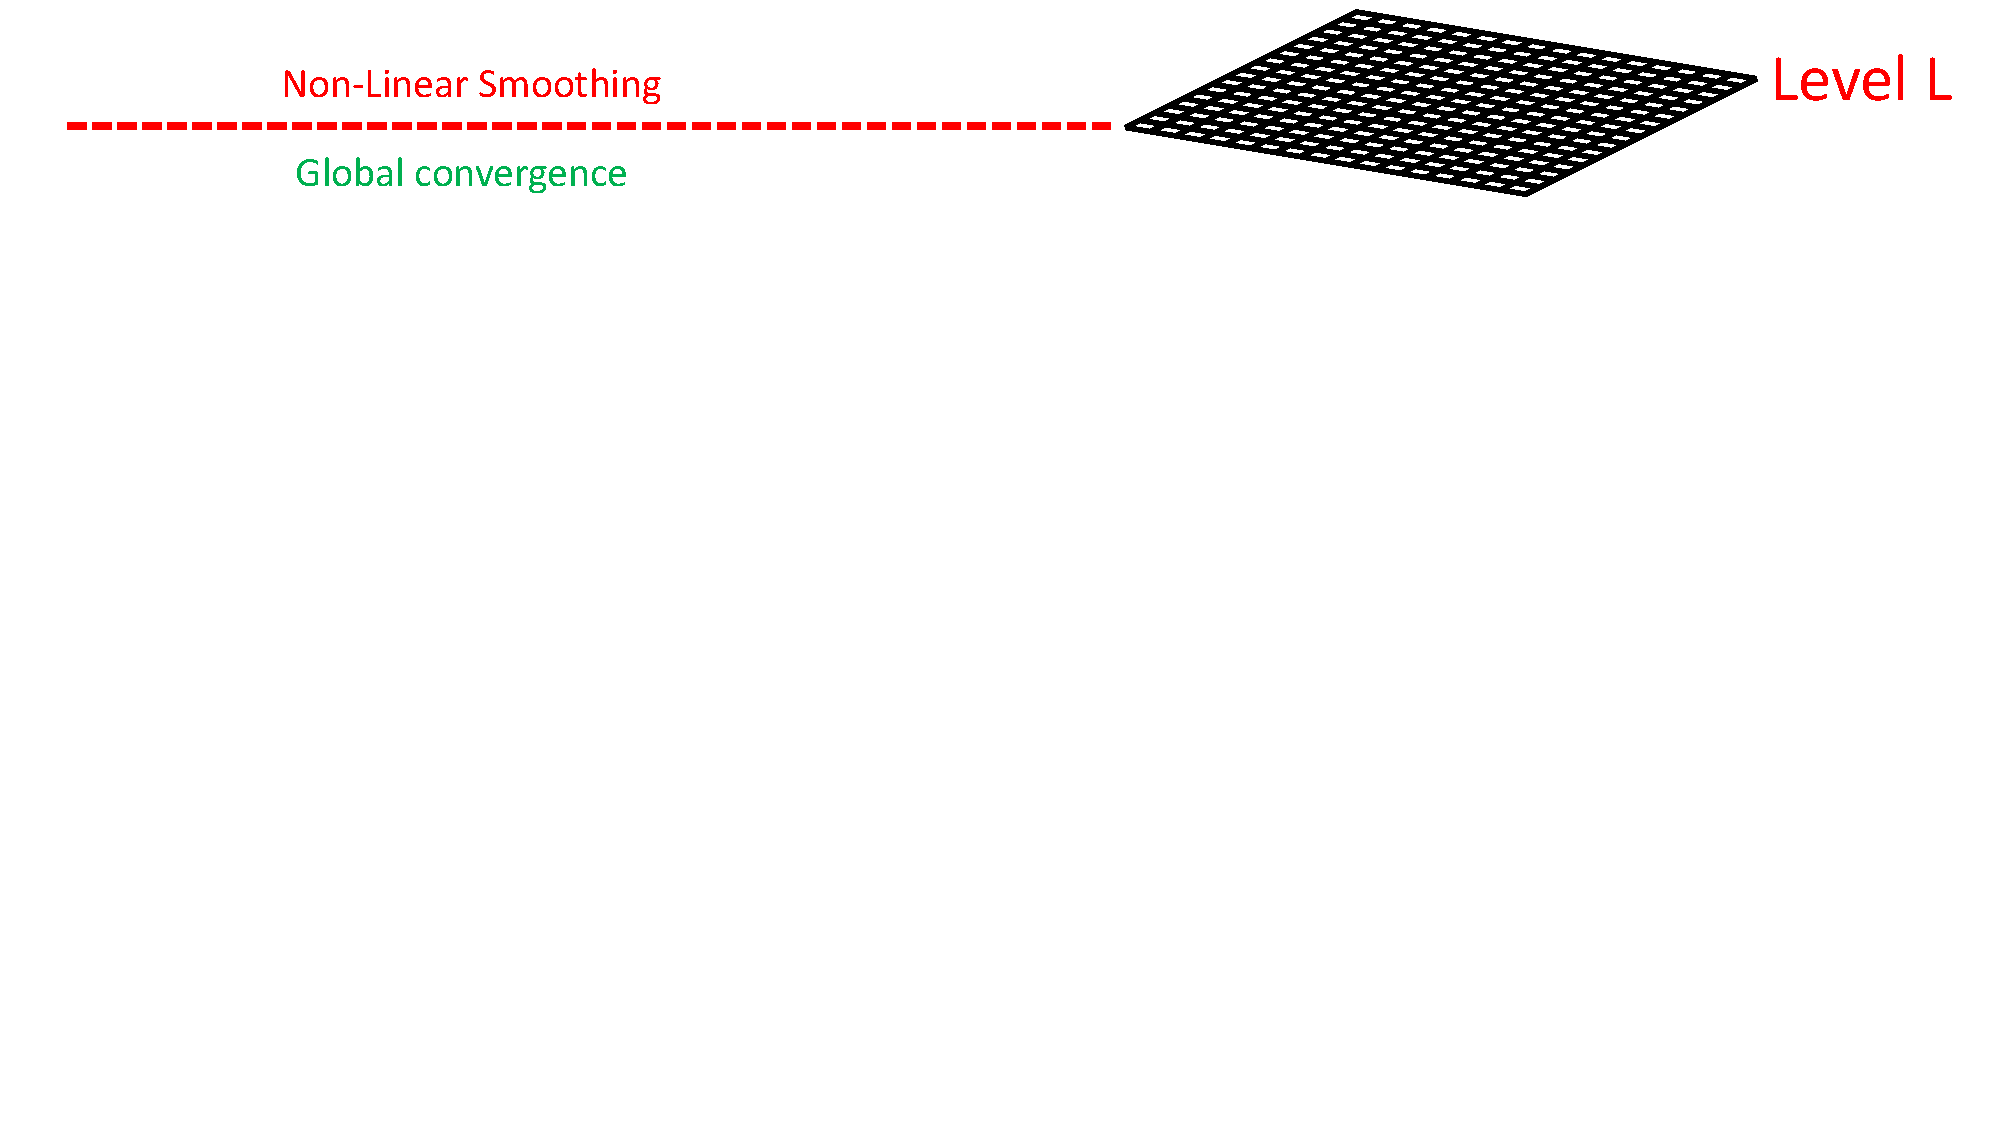
\includegraphics[width=1\textwidth]{img/multigridexplained1.pdf}
\end{figure}
\end{frame}

\begin{frame}
\titlecolor{Monotone Multilevel by energy minimization}
$R_{i}^{i-1}$ restriction operator ($ i=J,...,2 $)
\begin{figure}[htbp!]
		\centering
	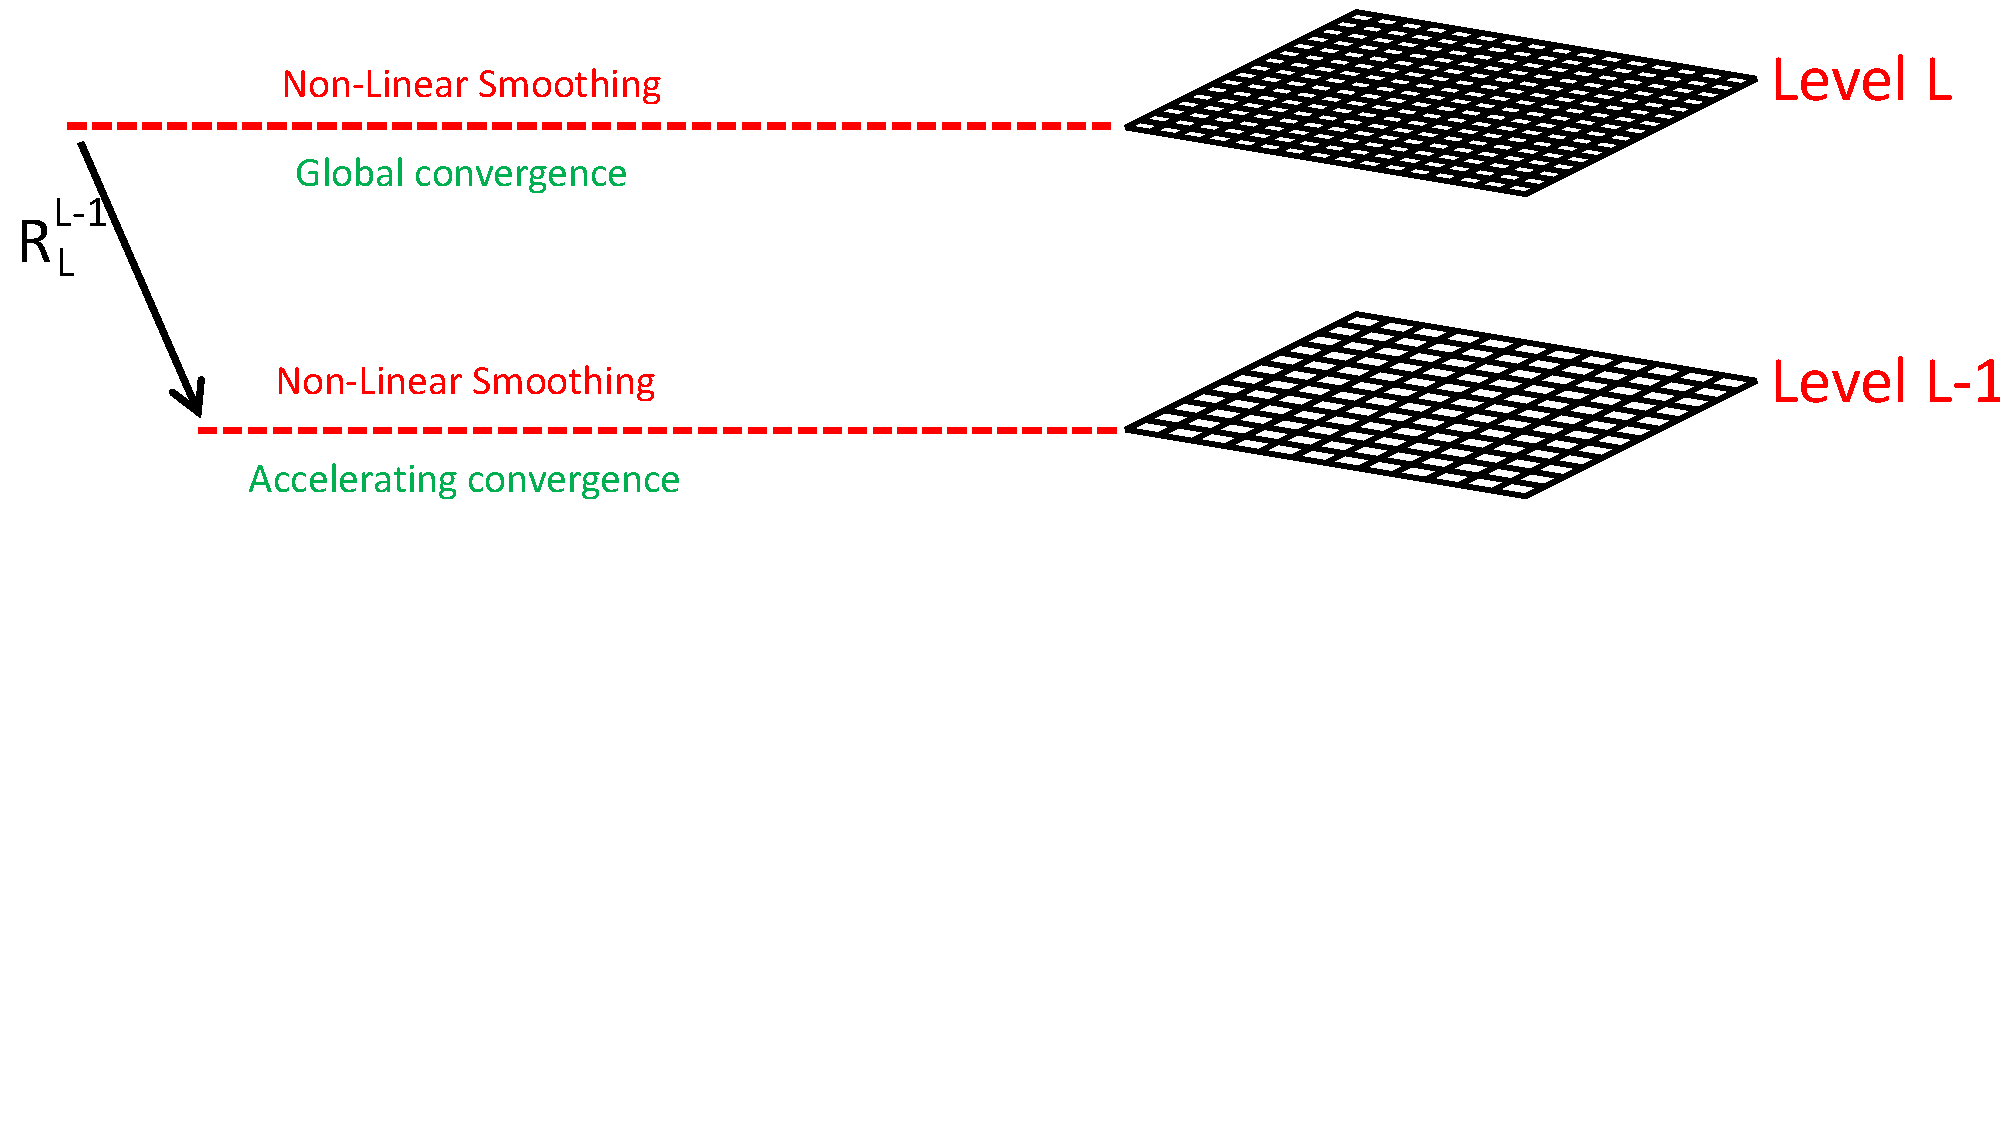
\includegraphics[width=1\textwidth]{img/multigridexplained2.pdf}
\end{figure}
\end{frame}

\begin{frame}
\titlecolor{Monotone Multilevel by energy minimization}
$R_{i}^{i-1}$ restriction operator ($ i=J,...,2 $)
\begin{figure}[htbp!]
		\centering
	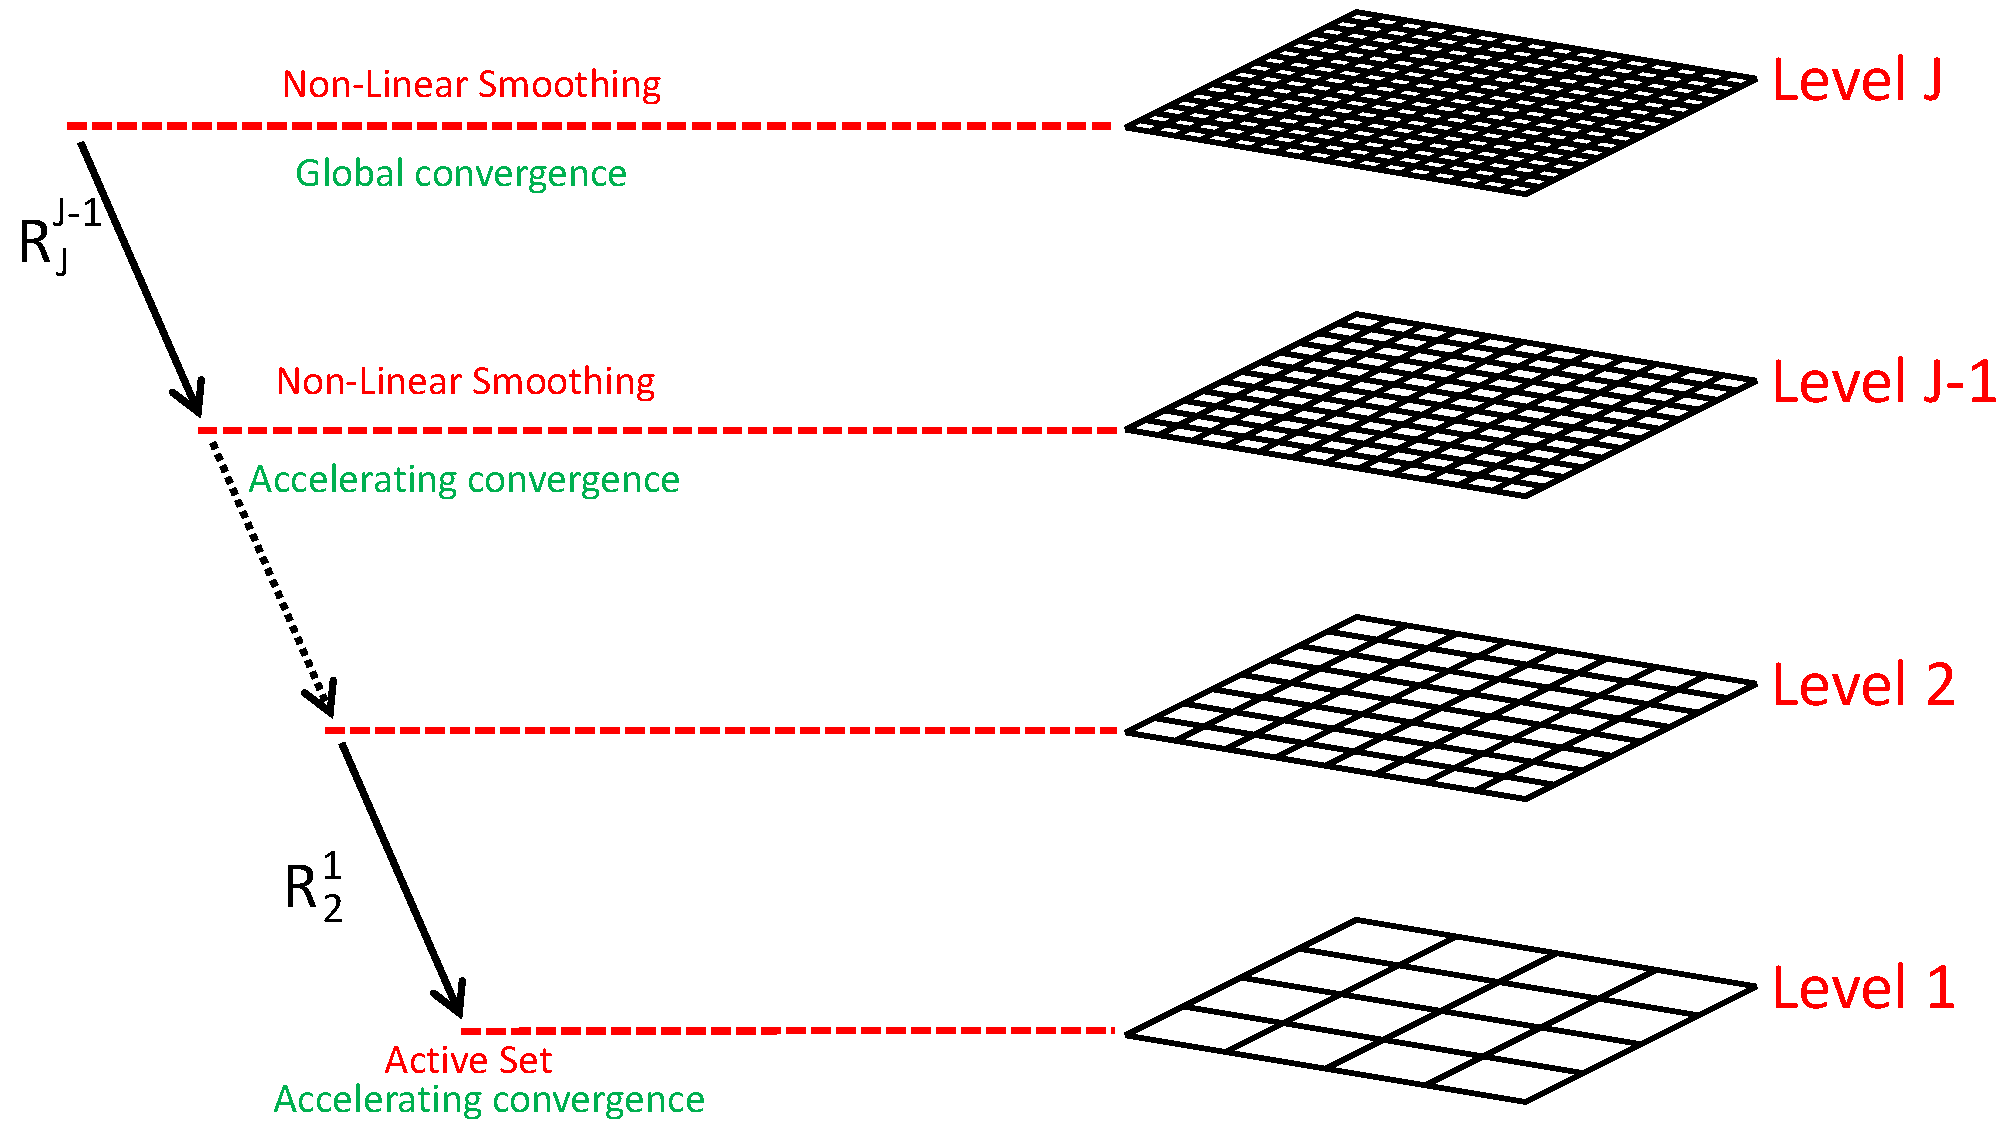
\includegraphics[width=1\textwidth]{img/multigridexplained3.pdf}
\end{figure}
\end{frame}
\begin{frame}
\titlecolor{Monotone Multilevel by energy minimization}
$R_{i}^{i-1}$ restriction operator, $I_{i-1}^{i}$ interpolation operator ($ i=J,...,2 $)
\begin{figure}[htbp!]
		\centering
	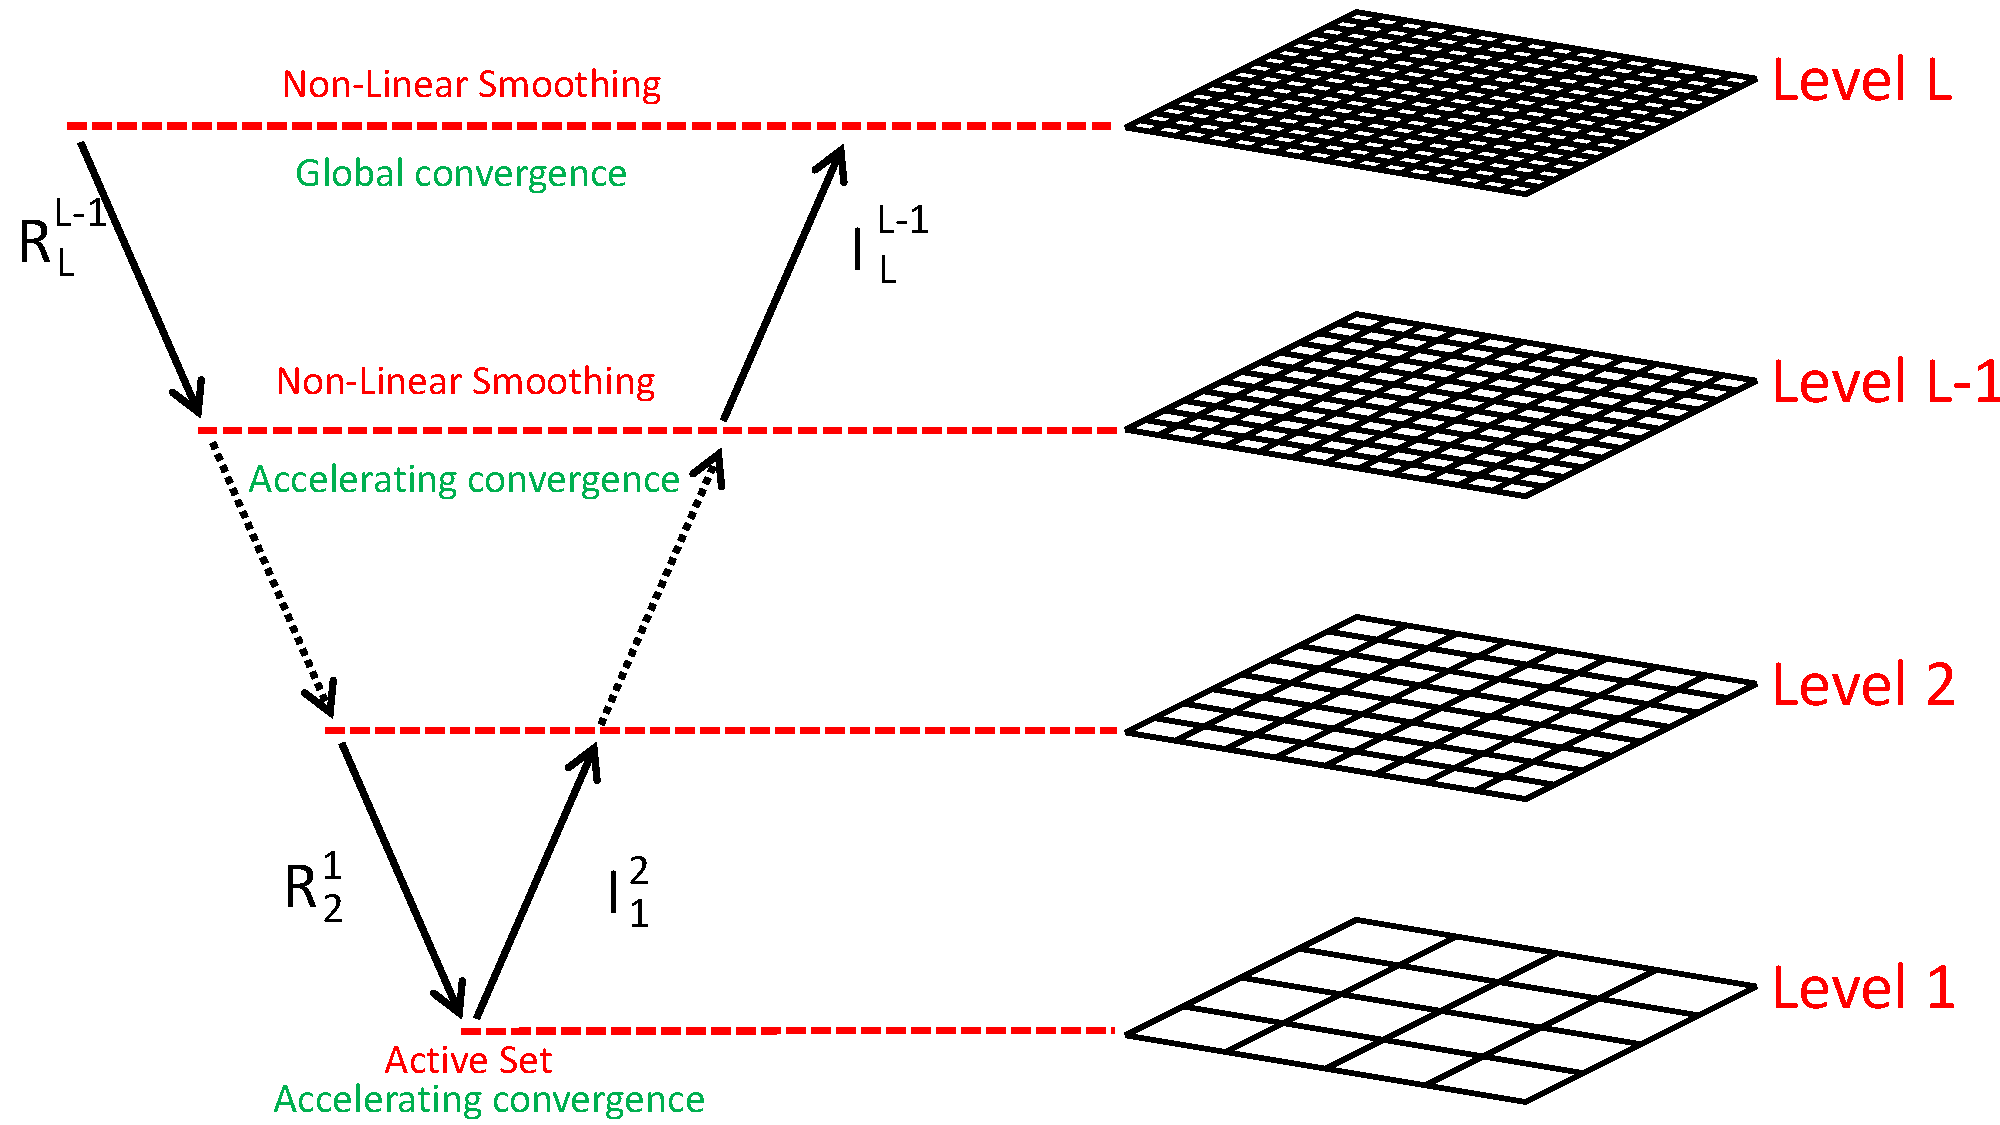
\includegraphics[width=1\textwidth]{img/multigridexplained4.pdf}
\end{figure}
\end{frame}



\begin{frame}
\titlecolor{Multilevel ingredients}
\textbf{Smoother}
\begin{itemize}
\item Standard non-linear Gau{\ss}-Seidel smooths $H^1$, \textbf{but not} $H_{\text{div}}$ 
\item The kernel $\text{Ker}(\text{div})=  \left\lbrace \btau \in H_{\text{div}}, \tdiv \btau =0   \right\rbrace $ is too large
\item  Patch-smoother \colk for divergence-free components of the error
\end{itemize}
${}$\\${}$\\
\textbf{Interpolations and restrictions}
\begin{itemize}
\item  Standard $P^1$ and $RT_0$ interpolations and restrictions for primal and dual variables
\item Non-linear projections for  constraint representation on coarser levels \colk
\end{itemize}
\end{frame}

\begin{frame}
\titlecolor{Multilevel ingredients}
\textbf{Smoother}
\begin{itemize}
\item Standard non-linear Gau{\ss}-Seidel smooths $H^1$, \textbf{but not} $H_{\text{div}}$ 
\item The kernel $\text{Ker}(\text{div})=  \left\lbrace \btau \in H_{\text{div}}, \tdiv \btau =0   \right\rbrace $ is too large
\item \colo \textbf{Patch-smoother} \colk for divergence-free components of the error
\end{itemize}
${}$\\${}$\\
\textbf{Interpolations and restrictions}
\begin{itemize}
\item  Standard $P^1$ and $RT_0$ interpolations and restrictions for primal and dual variables
\item Non-linear projections for constraint representation on coarser levels \colk
\end{itemize}
\end{frame}






%%%%%%%%%%%%%%%%%%%%%%%%%%%%%%%%%%%%%%%%%%
%%%%%%%%%%%                   SLIDE 5                %%%%%%%%%%%%%%%
%%%%%%%%%%%%%%%%%%%%%%%%%%%%%%%%%%%%%%%%%%



%%%%%%%%%%%%%%%%%%%%%%%%%%%%%%%%%%%%%%%%%%
%%%%%%%%%%%                   SLIDE 6                %%%%%%%%%%%%%%%
%%%%%%%%%%%%%%%%%%%%%%%%%%%%%%%%%%%%%%%%%%

\begin{frame}
\titlecolor{LS Patch smoother}
\footnotesize

\begin{figure}[htbp!]
	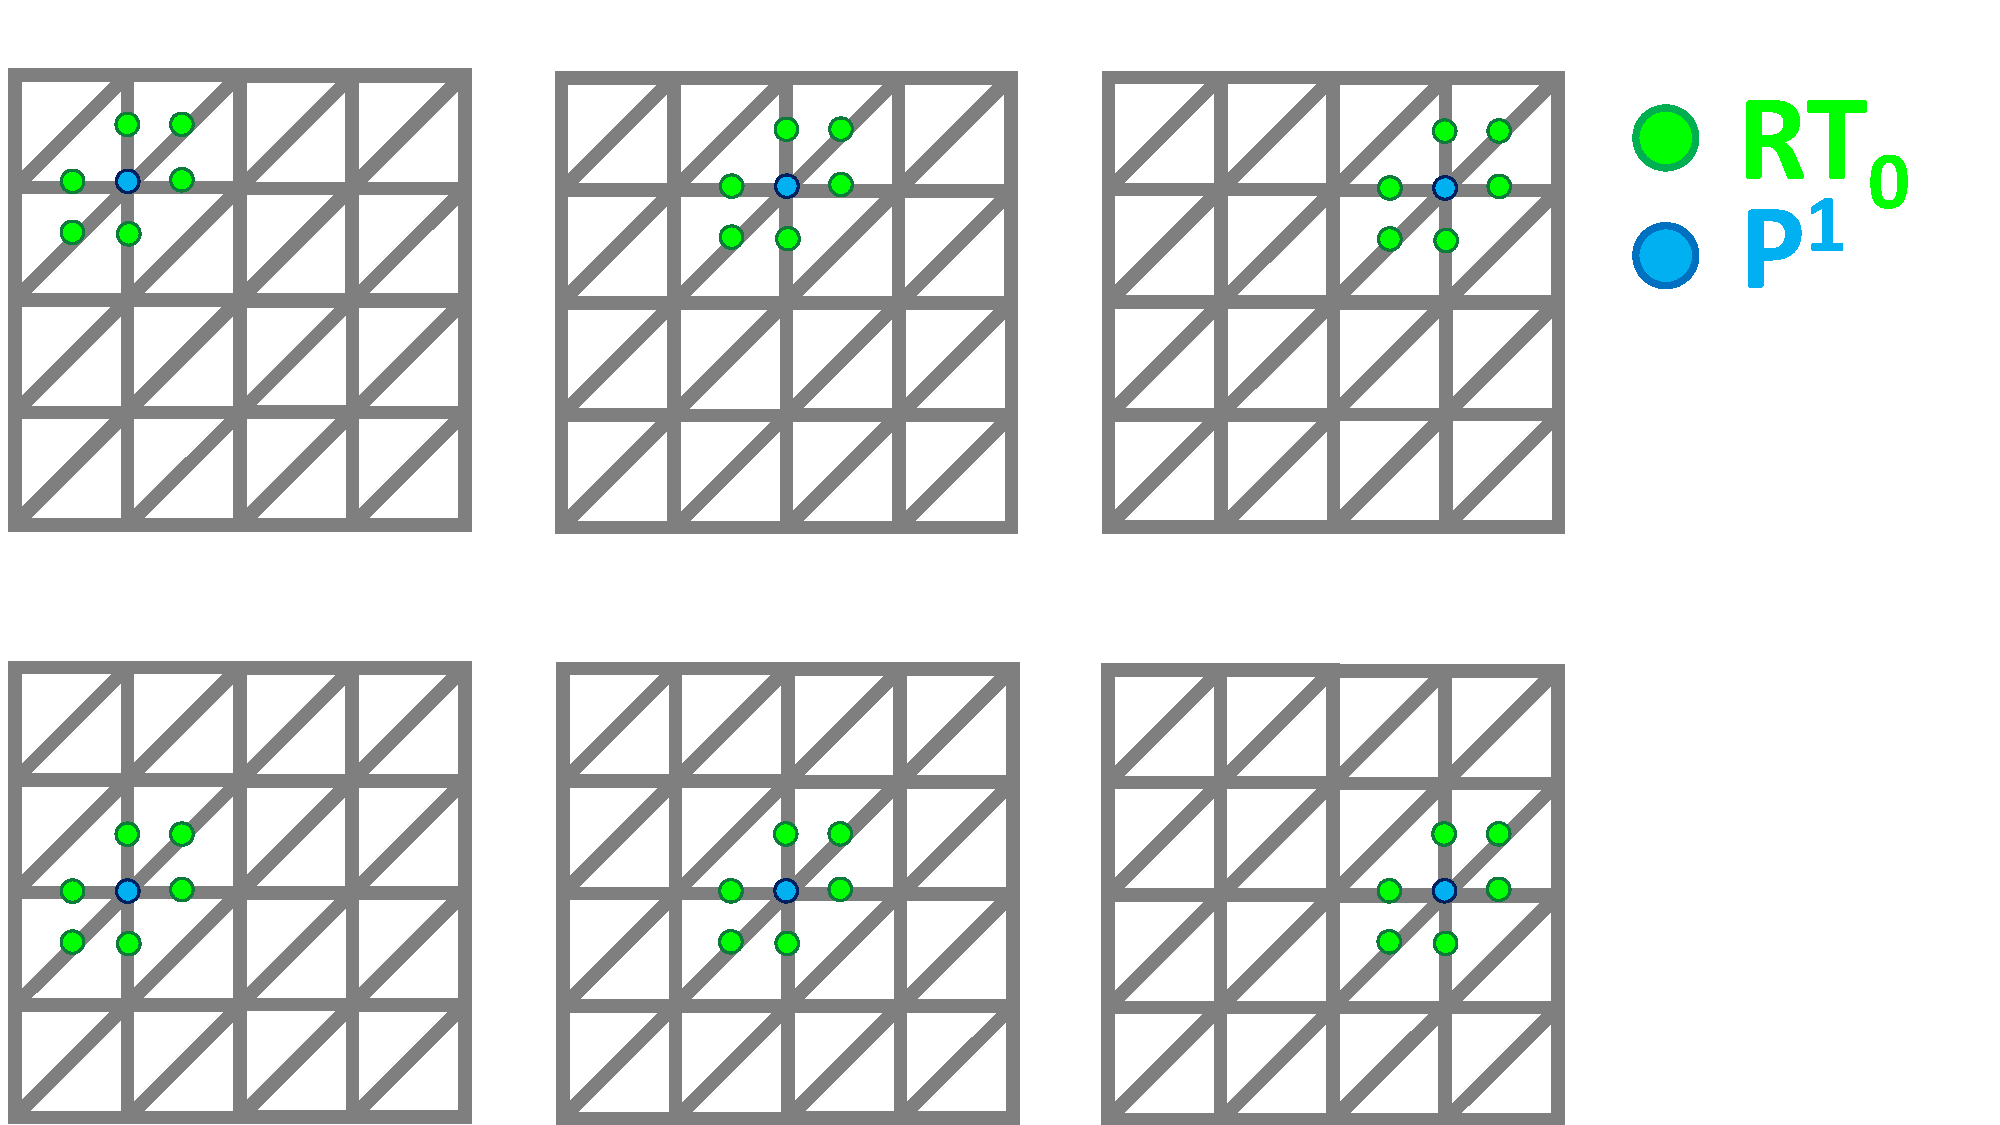
\includegraphics[width=0.8\textwidth]{img/patchsmoother.pdf}
		\label{abb_arc}
\end{figure}
$\bullet$ Minimization of $\mathcal{J}(\bu,\bsigma)$ on $\text{span}(\lambda_{j,\nu})$\\
$\bullet$ Exploit $\nu$-patches to smooth the error in $H^1$ and $H_{\text{div}}$ simultaneously\\
${}$\\
\tiny{Ralf Hiptmair. Multigrid method for H(div) in three dimensions. Electron. Trans. Numer. Anal, 6(1):133-152, 1997.}${}$\\
${}$\\
\tiny{Douglas N Arnold, Richard S Falk, and Ragnar Winther. Multigrid in H(div) and H(curl). Numerische Mathe-
matik, 85(2):197-217, 2000.}
${}$\\
${}$\\
\tiny{
Gerhard Starke. Gauss-Newton multilevel methods for least-squares finite element computations of variably saturated subsurface flow. Computing, 64(4):323-338, 2000.}

\end{frame}










\begin{frame}
\titlecolor{Multilevel ingredients}
\textbf{Smoother}
\begin{itemize}
\item Standard non-linear Gau{\ss}-Seidel smooths $H^1$, \textbf{but not} $H_{\text{div}}$ 
\item The kernel $\text{Ker}(\text{div})=  \left\lbrace \btau \in H_{\text{div}}, \tdiv \btau =0   \right\rbrace $ is too large
\item Patch-smoother \colk for divergence-free components of the error
\end{itemize}
${}$\\${}$\\
\textbf{Interpolations and restrictions}
\begin{itemize}
\item  Standard $P^1$ and $RT_0$ interpolations and restrictions for primal and dual variables
\item Non-linear projections for \colo \textbf{constraint representation on coarser levels} \colk
\end{itemize}
\end{frame}

%%%%%%%%%%%%%%%%%%%%%%%%%%%%%%%%%%%%%%%%%%
%%%%%%%%%%%                   SLIDE 7                %%%%%%%%%%%%%%%
%%%





%%%%%%%%%%%%%%%%%%%%%%%%%%%%%%%%%%%%%%%%%%
%%%%%%%%%%%                   SLIDE 10               %%%%%%%%%%%%%%%
%%%%%%%%%%%%%%%%%%%%%%%%%%%%%%%%%%%%%%%%%%

\begin{frame}
\titlecolor{Non-Linear Projections for Coarse Constraints}
\begin{itemize}
\item {\colgold Wrong} and {\colg correct} coarse constraints
\begin{figure}[htbp!]
		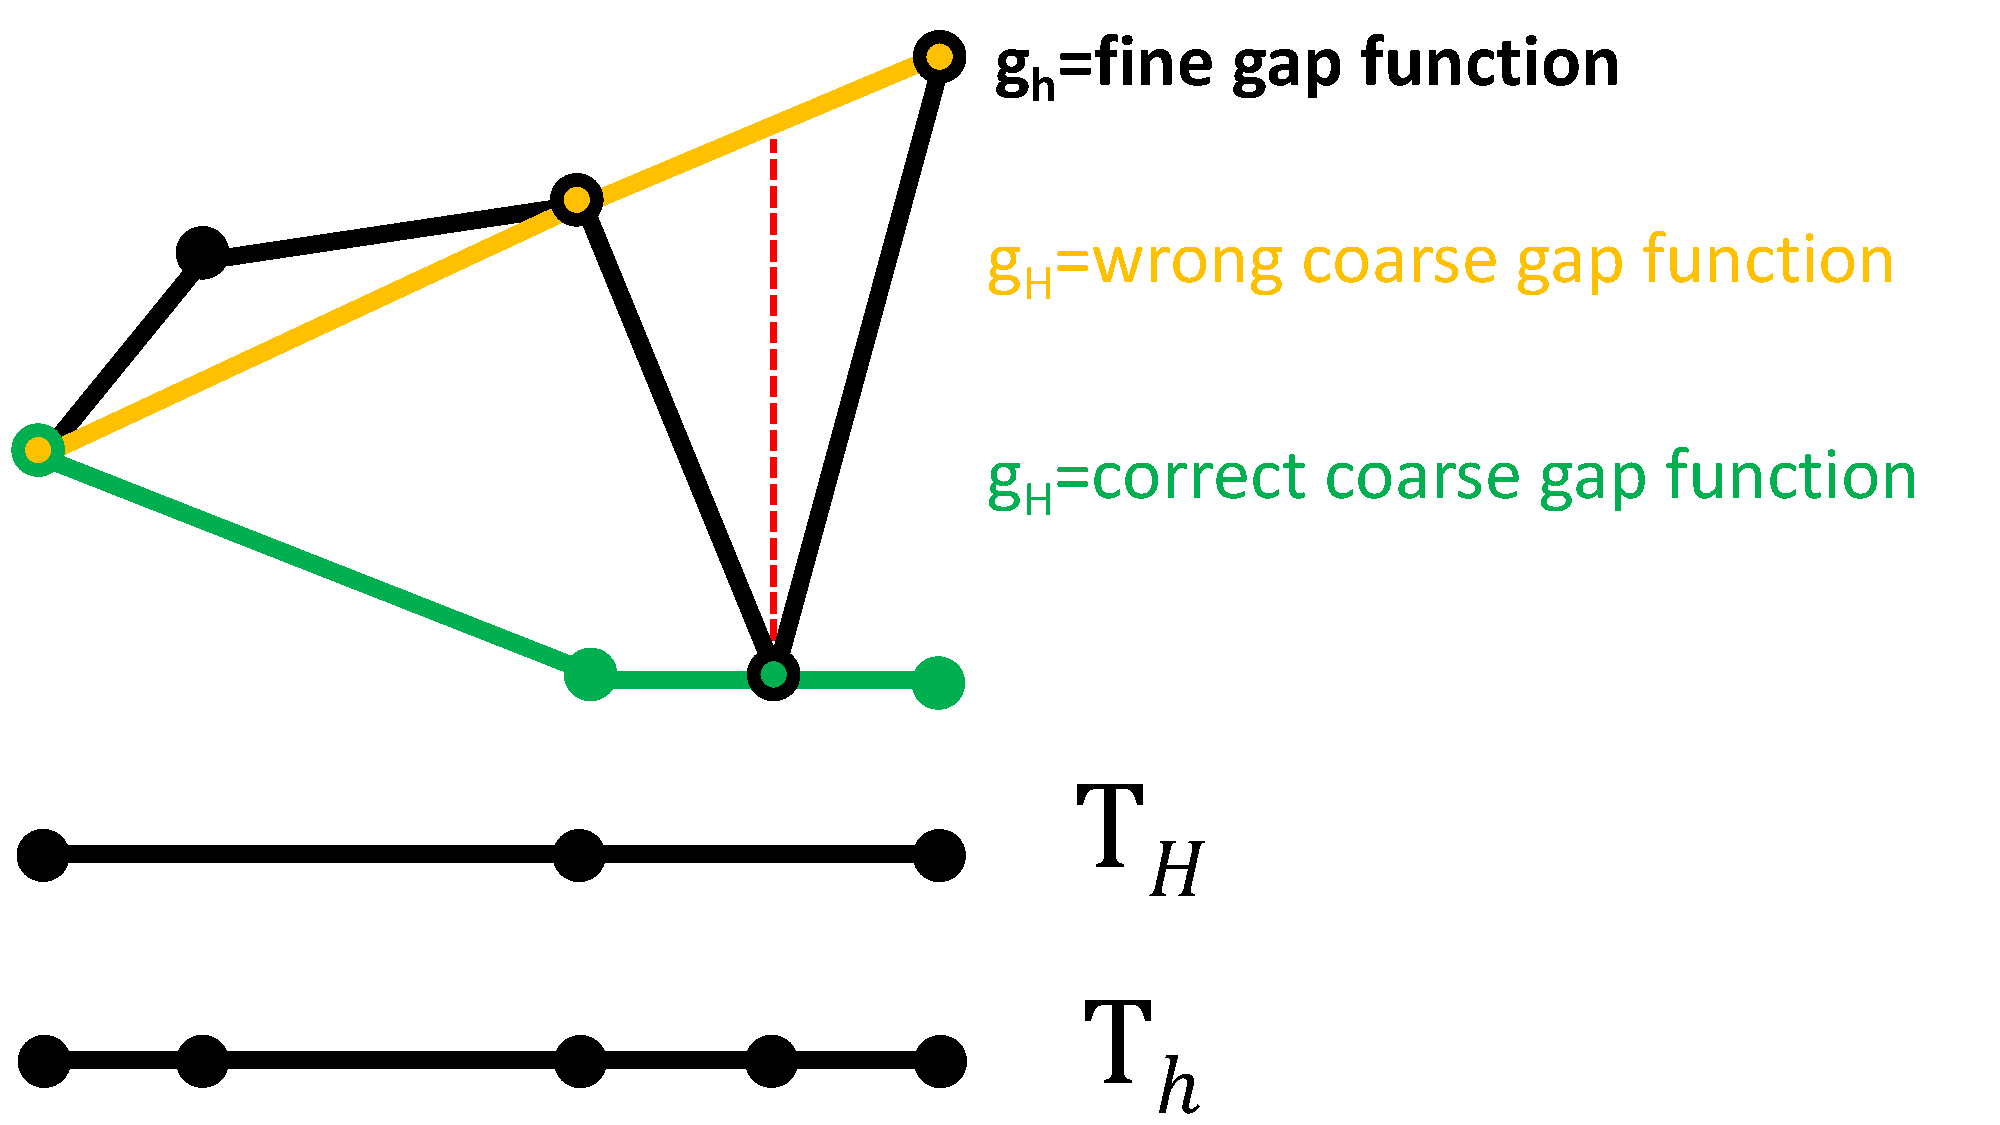
\includegraphics[scale=0.15]{img/coarseconstraintrepresentation.pdf}
\end{figure}
\item Different consistent coarse constraints
\begin{figure}[htbp!]
		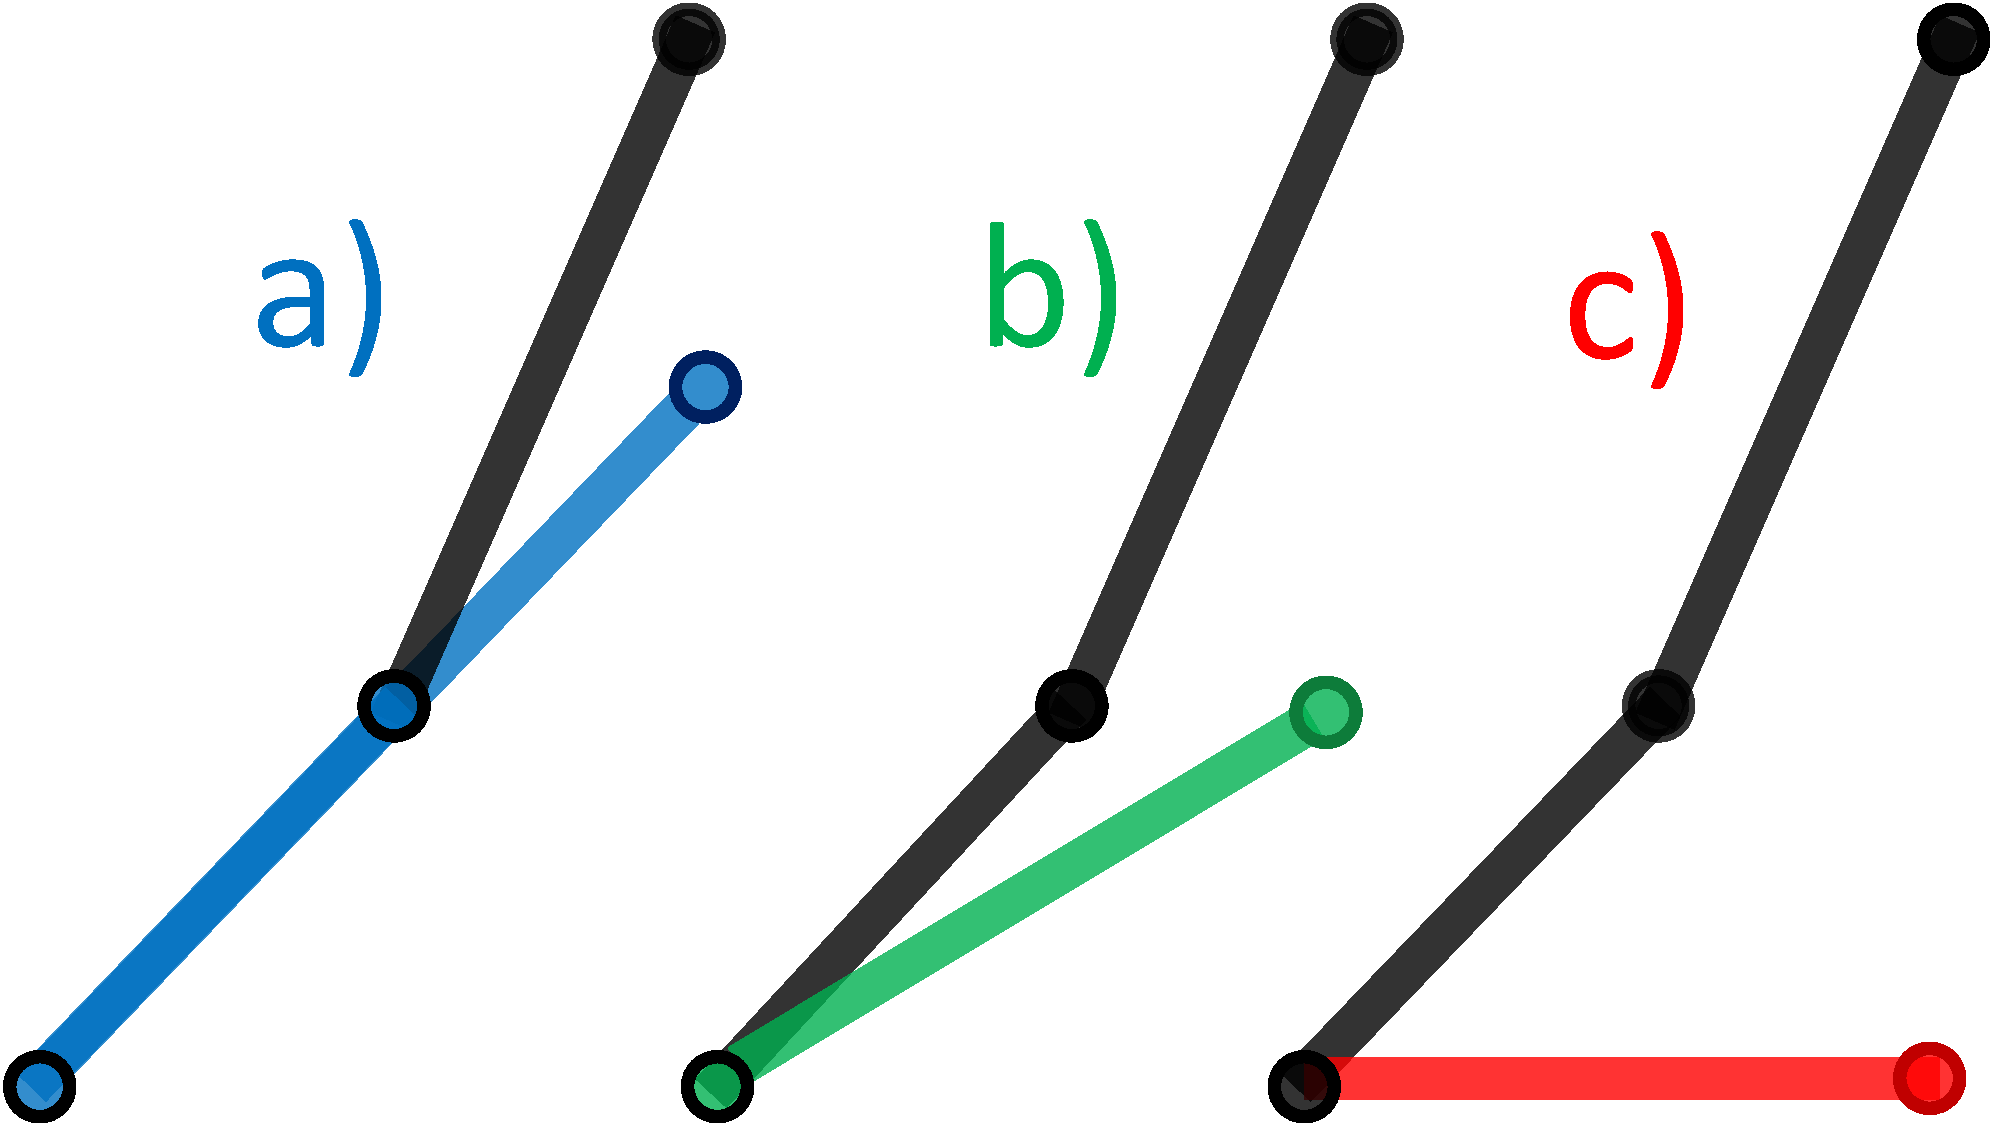
\includegraphics[scale=0.11]{img/coarseconstraintabc.pdf}
\end{figure}
\end{itemize}
\end{frame}


%%%%%%%%%%%%%%%%%%%%%%%%%%%%%%%%%%%%%%%%%%
%%%%%%%%%%%                   SLIDE 11               %%%%%%%%%%%%%%%
%%%%%%%%%%%%%%%%%%%%%%%%%%%%%%%%%%%%%%%%%%
\begin{frame}
\titlecolor{Hertzian Contact - Setting}
\begin{figure}[htbp!]
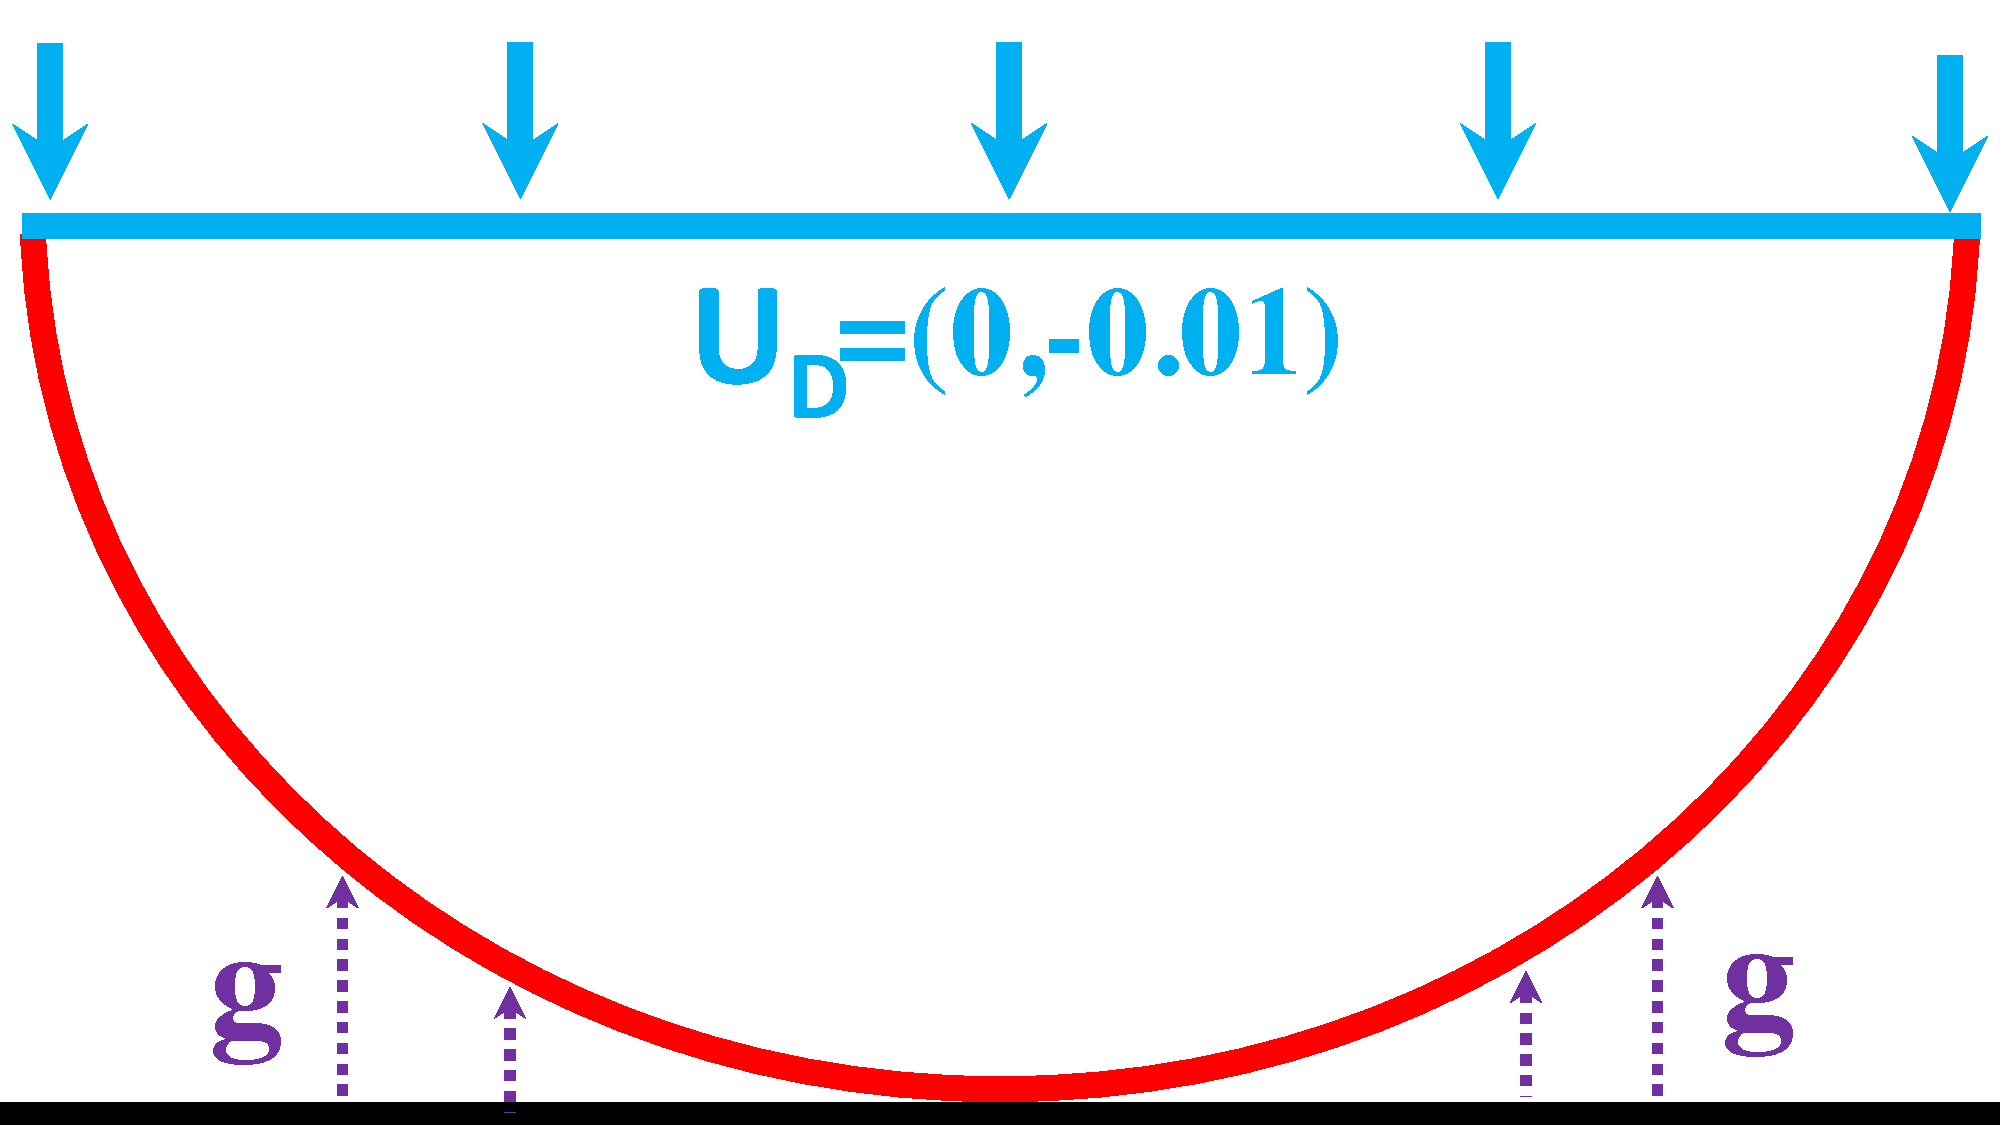
\includegraphics[scale=0.2]{img/signorinicircle.pdf} 
\end{figure}
$ \mu = 1$, $ \lambda = 1, \infty$ (compressible and \textbf{incompressible})
\end{frame}

%%%%%%%%%%%%%%%%%%%%%%%%%%%%%%%%%%%%%%%%%%
%%%%%%%%%%%                   SLIDE 12               %%%%%%%%%%%%%%%
%%%%%%%%%%%%%%%%%%%%%%%%%%%%%%%%%%%%%%%%%%

\begin{frame}
\titlecolor{Hertzian Contact, two-level problem}
\begin{figure}[htbp!]
	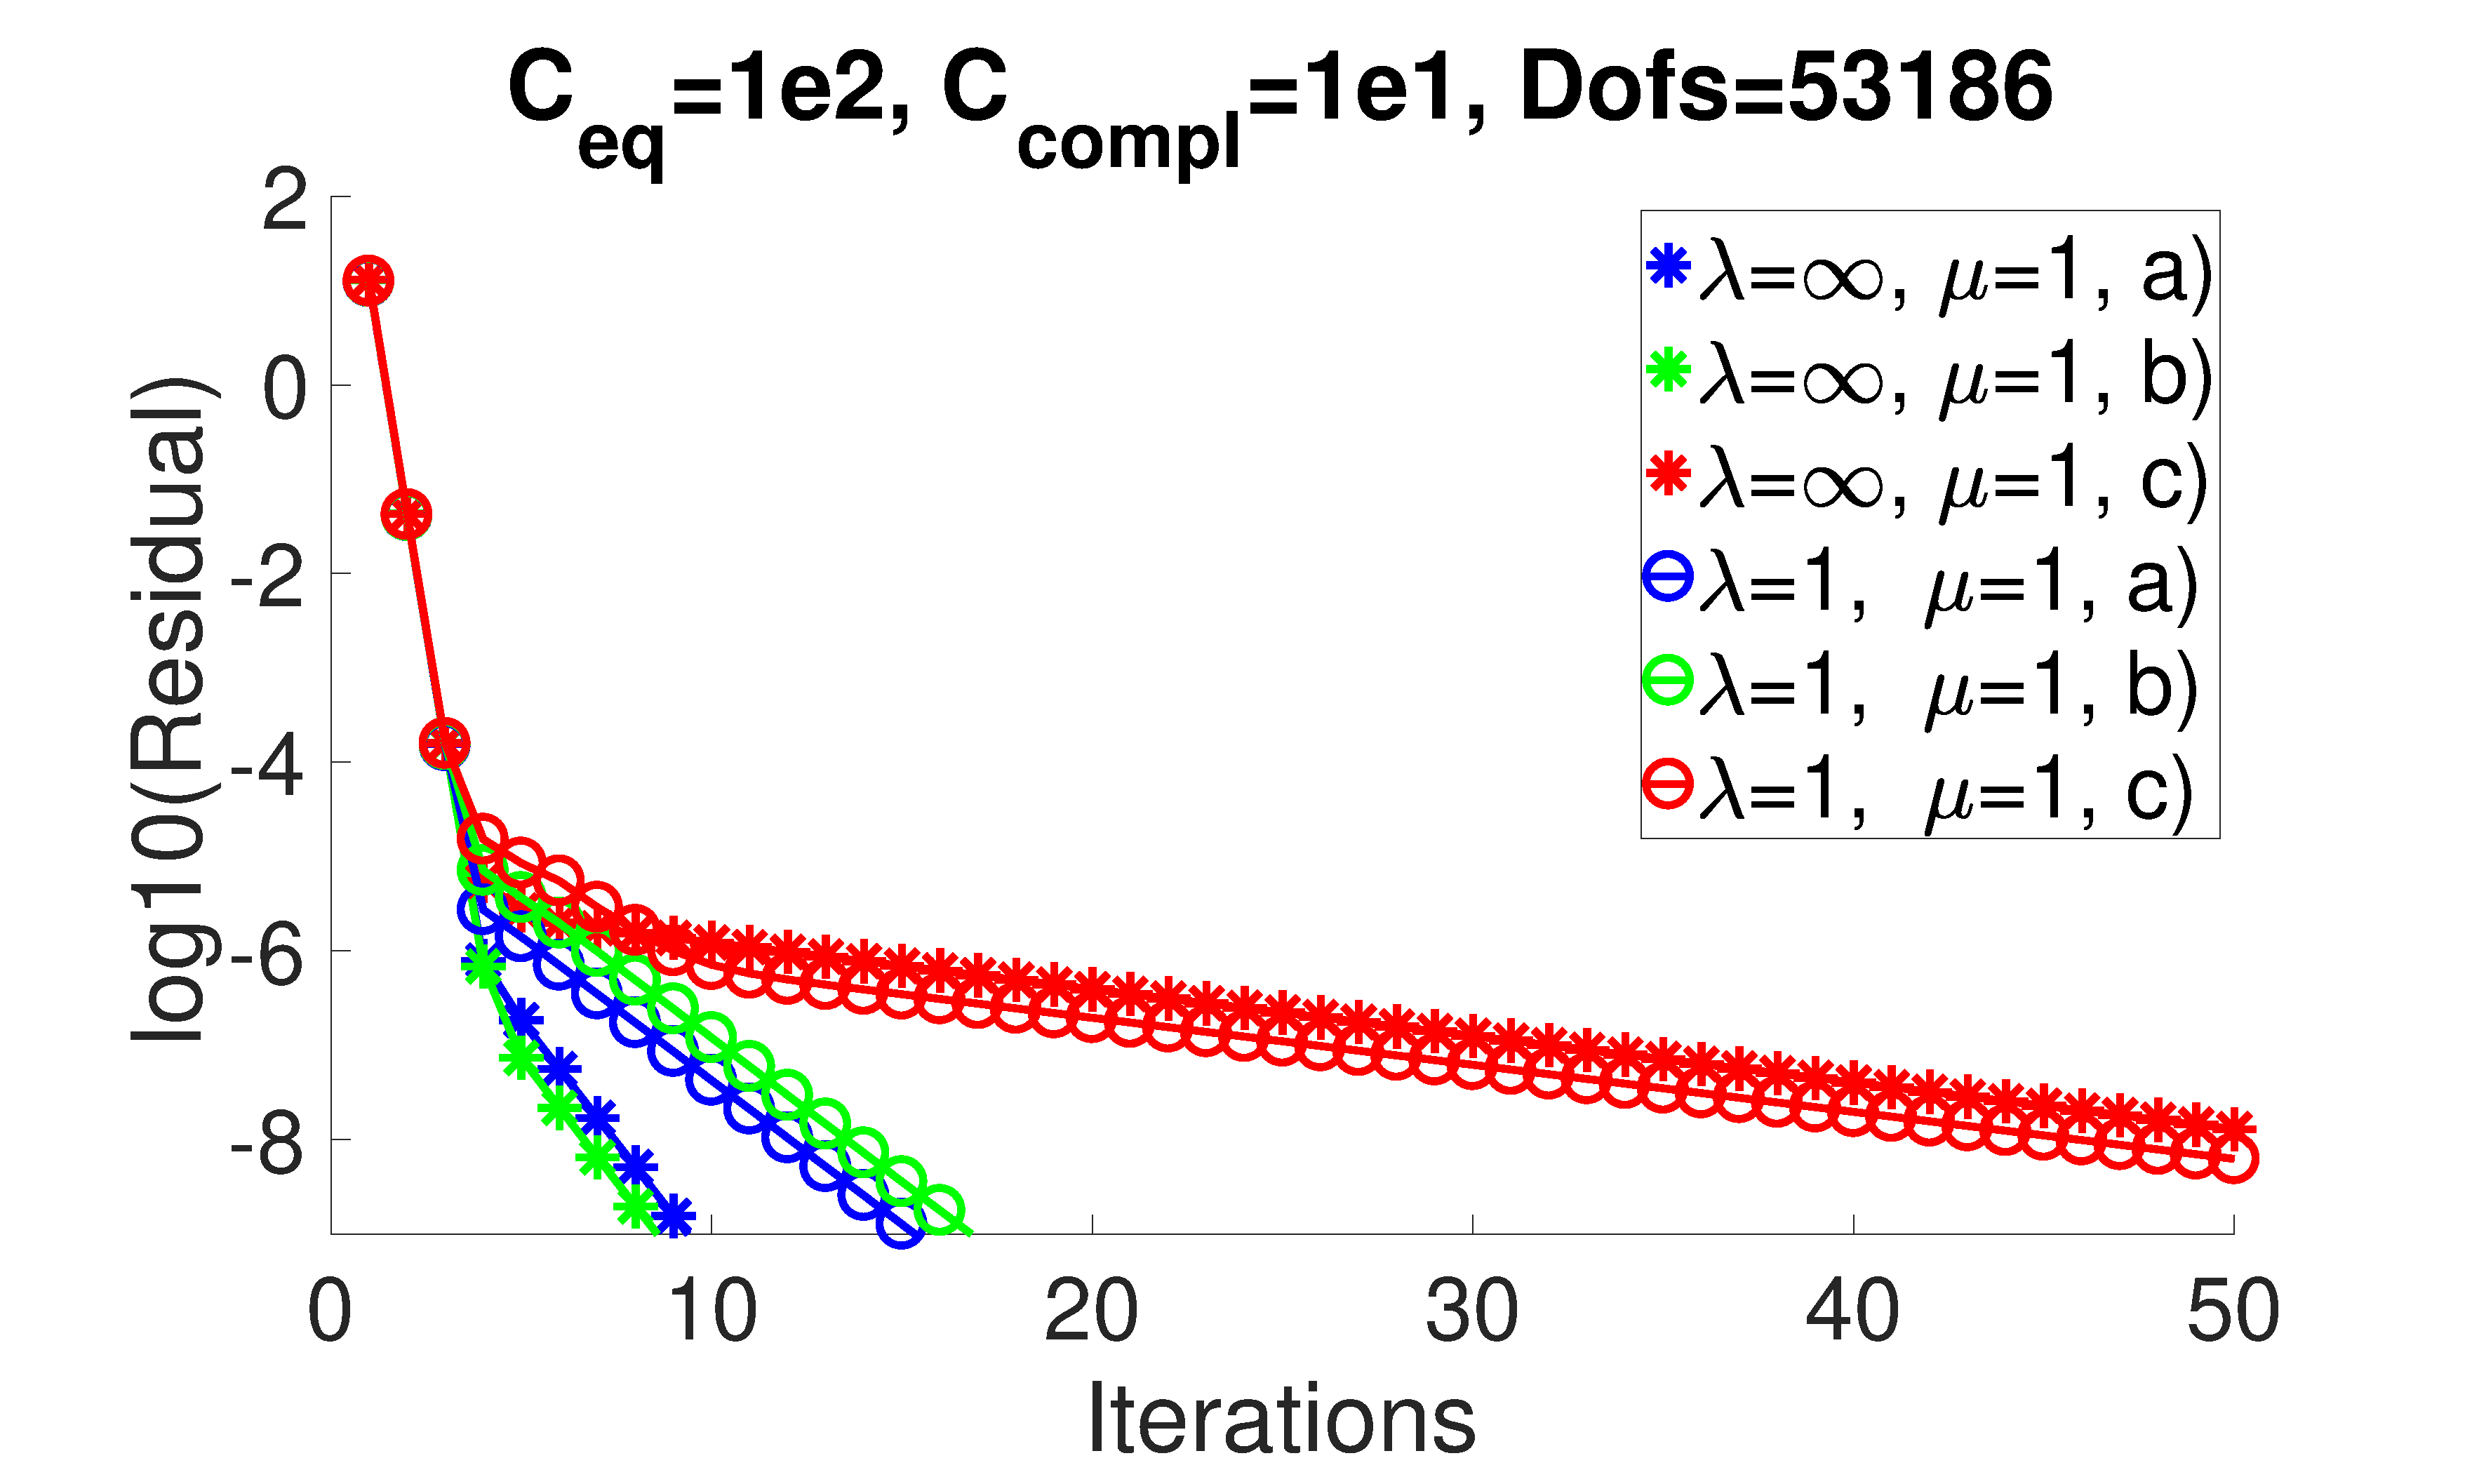
\includegraphics[scale=0.08]{img/ResidualsNonUniform.eps}
		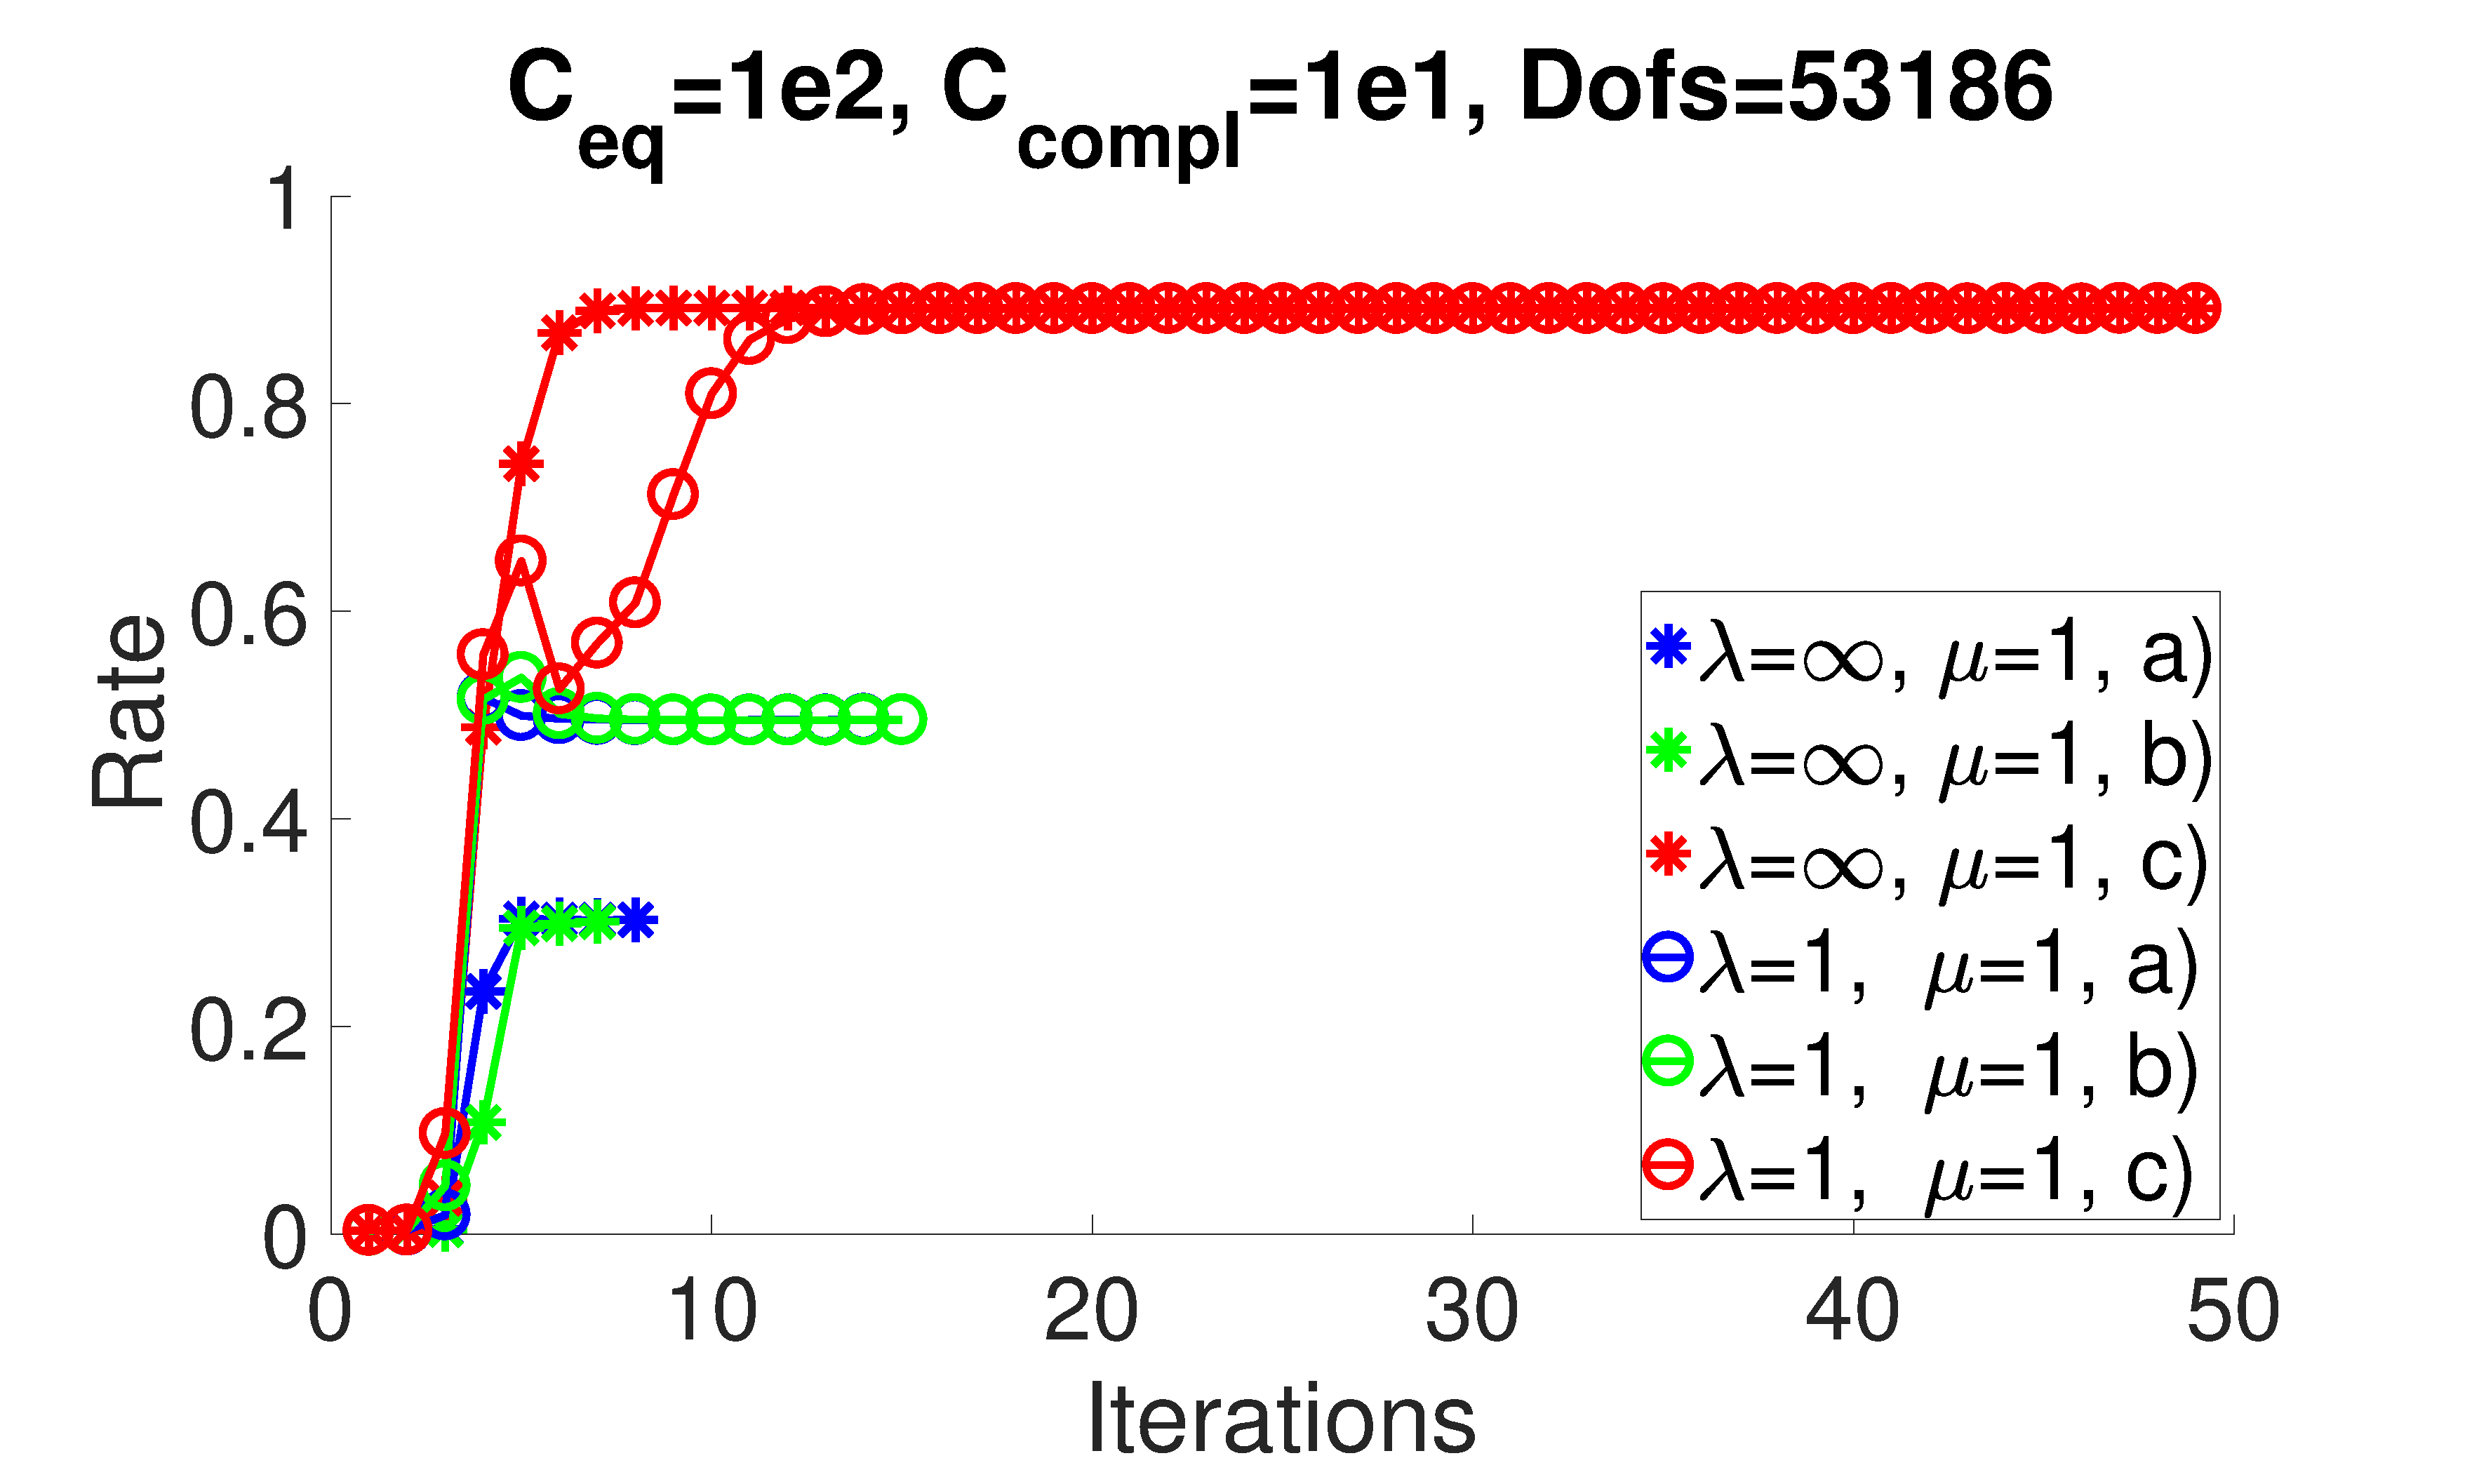
\includegraphics[scale=0.08]{img/RatesNonUniform.eps}
	\caption{Mesh with $h_{max}/h_{min}=7.0567$}
		\label{ResidualRateVeryNonUniform}
\end{figure}
\begin{itemize}
\item \textbf{First phase}: non-linear, capturing high frequencies
\item \textbf{Second phase}: linear, known active set (blue, green), and not already known active set(red)
\item  \textbf{Similar behaviour} of compressible and incompressible cases
\end{itemize}
\end{frame}


%%%%%%%%%%%%%%%%%%%%%%%%%%%%%%%%%%%%%%%%%%
%%%%%%%%%%%                   SLIDE 13               %%%%%%%%%%%%%%%
%%%%%%%%%%%%%%%%%%%%%%%%%%%%%%%%%%%%%%%%%%
\begin{frame}
\titlecolor{Hertzian Contact - Setting}
\begin{figure}[htbp!]
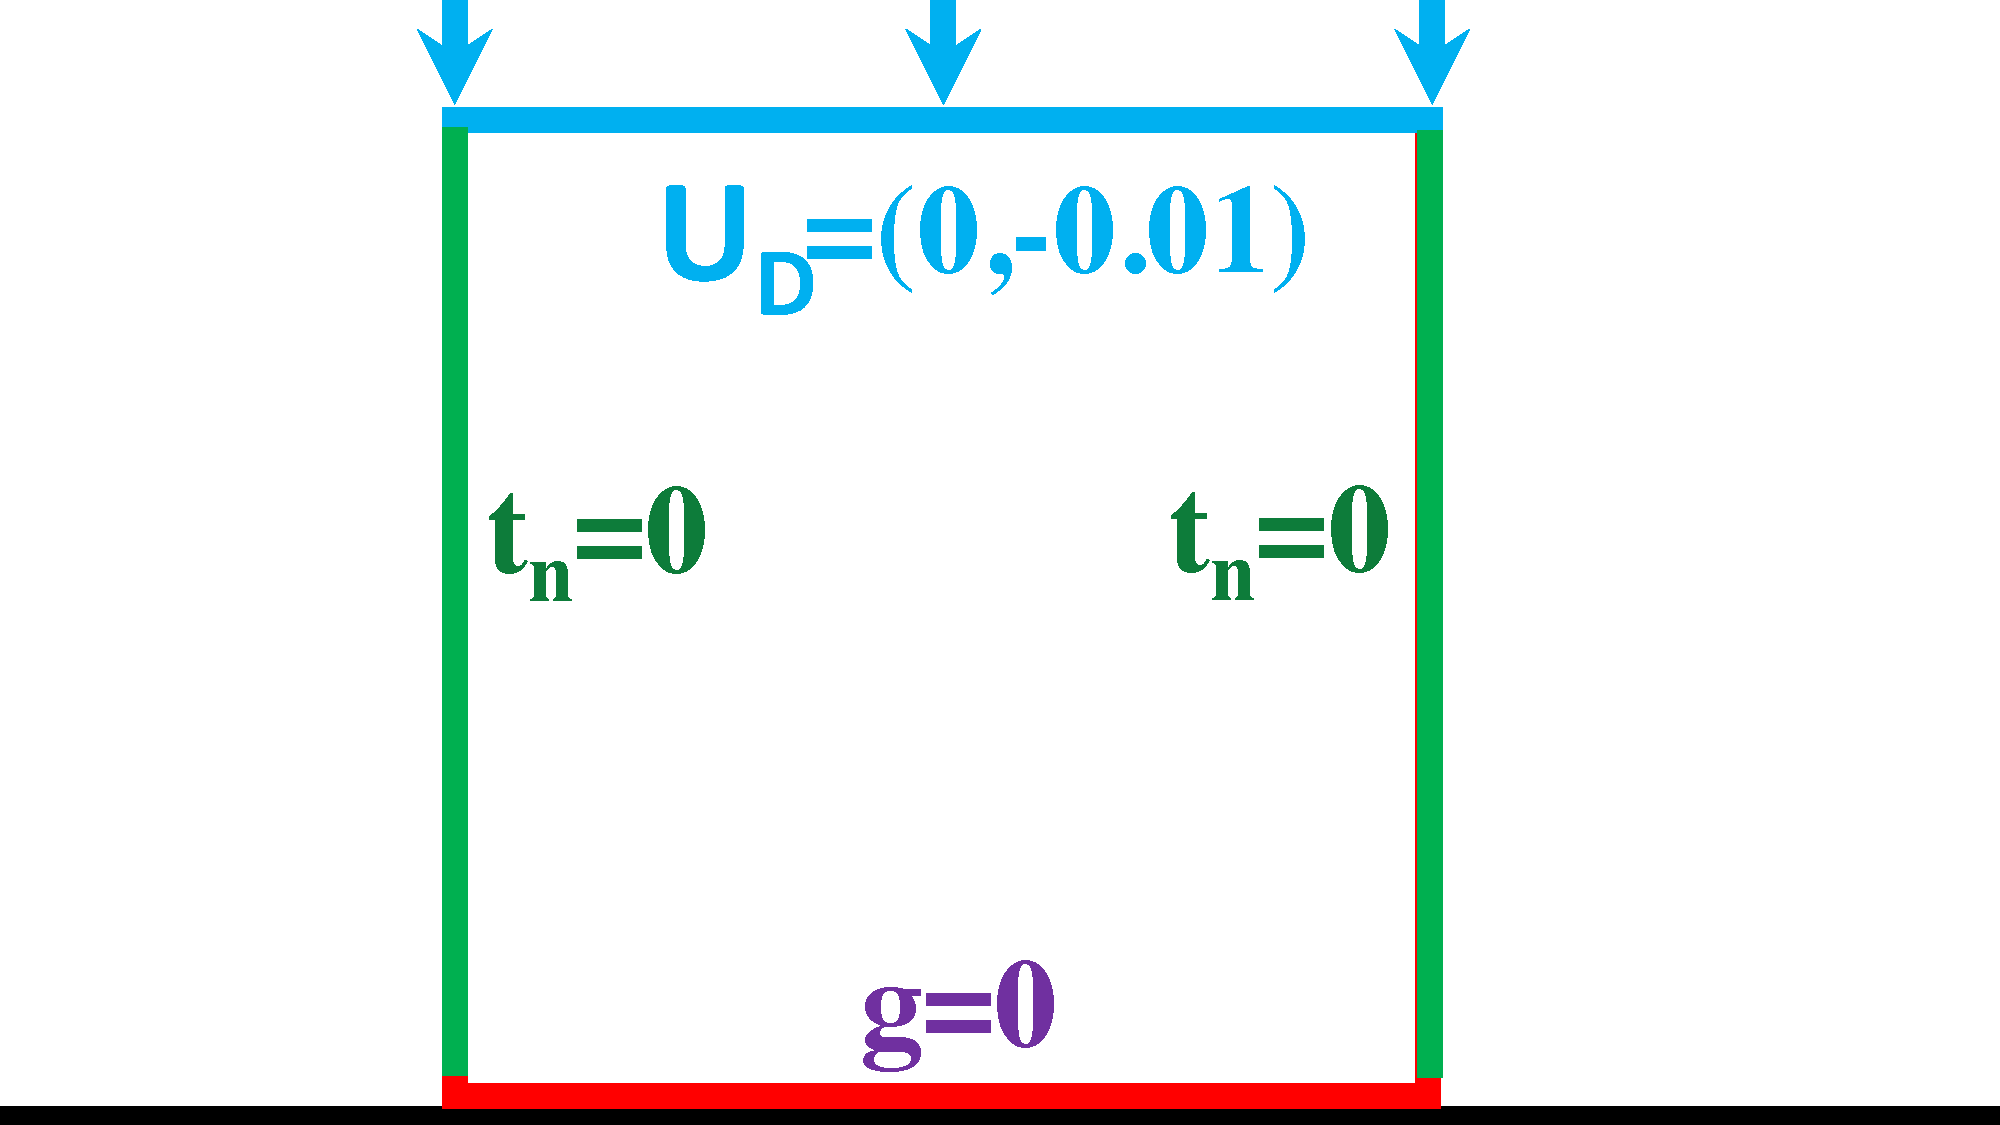
\includegraphics[scale=0.2]{img/signorinisquare.pdf} 
\end{figure}
$ \mu = 1$, $ \lambda = 1, \infty$ (compressible and \textbf{incompressible})
\end{frame}

\begin{frame}
\titlecolor{Signorini's problem, square mesh}
\footnotesize
\begin{figure}[htbp!]
	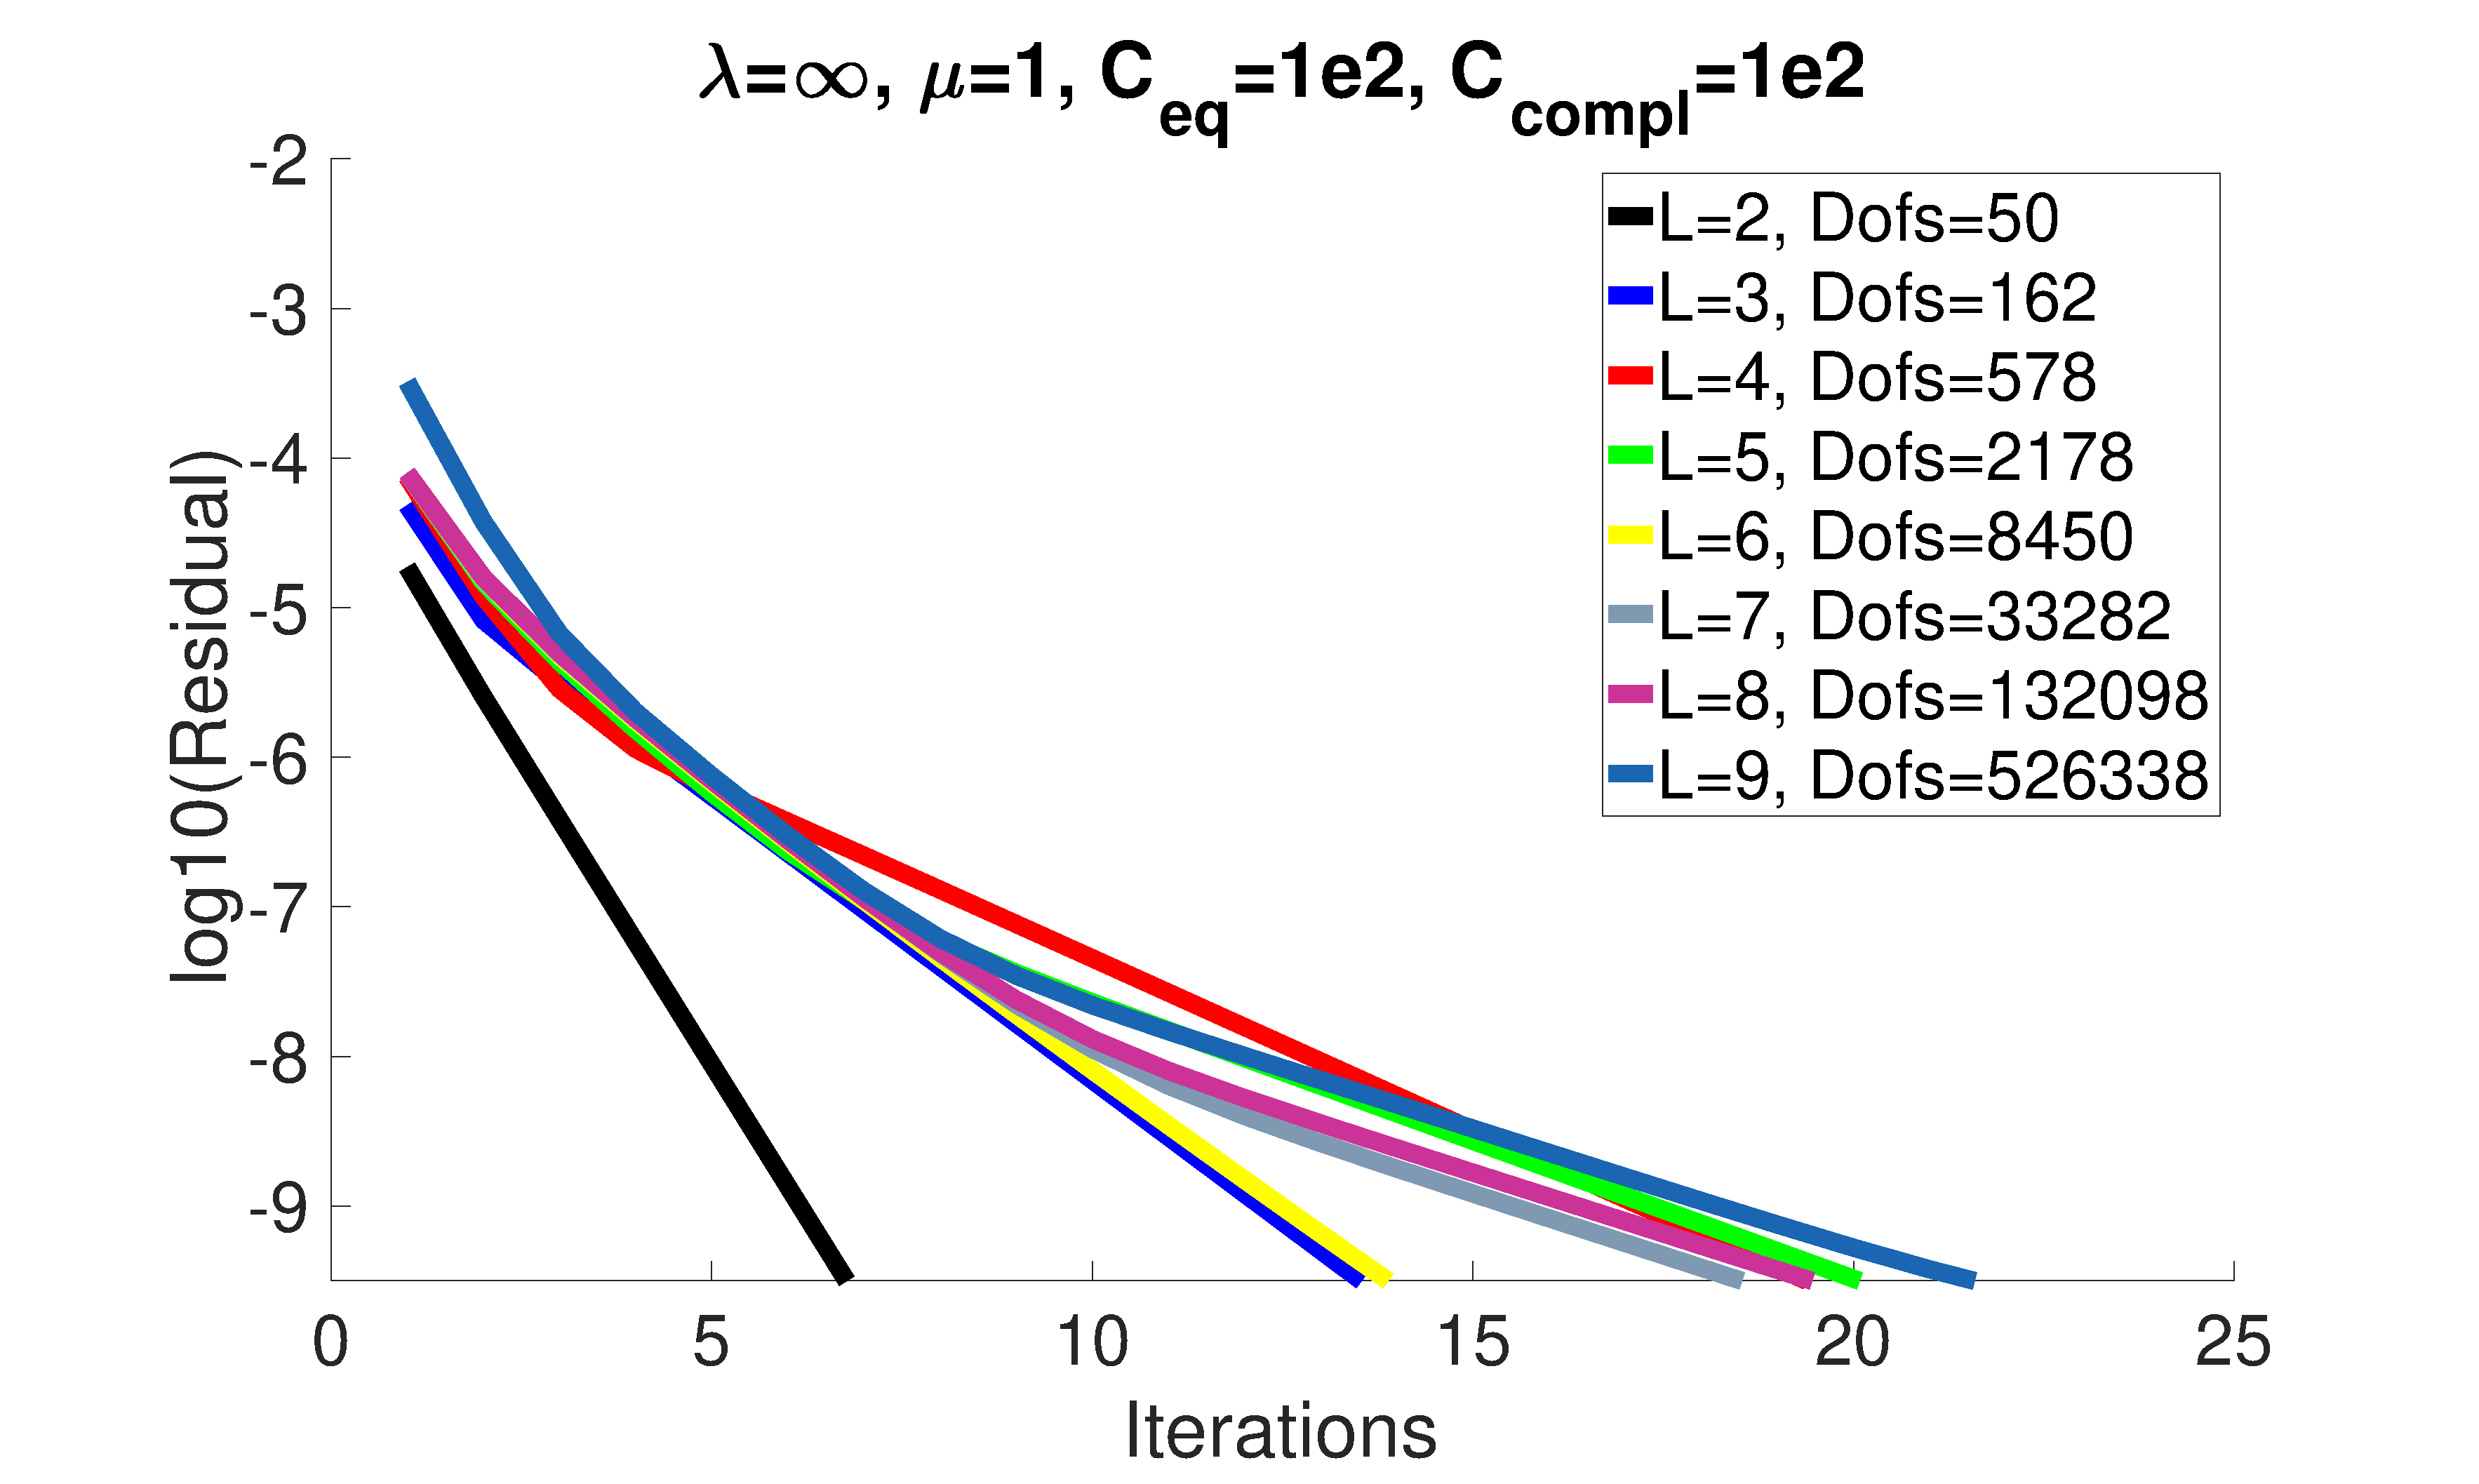
\includegraphics[scale=0.08]{img/SquareResidualCompressible.eps}
	\quad
		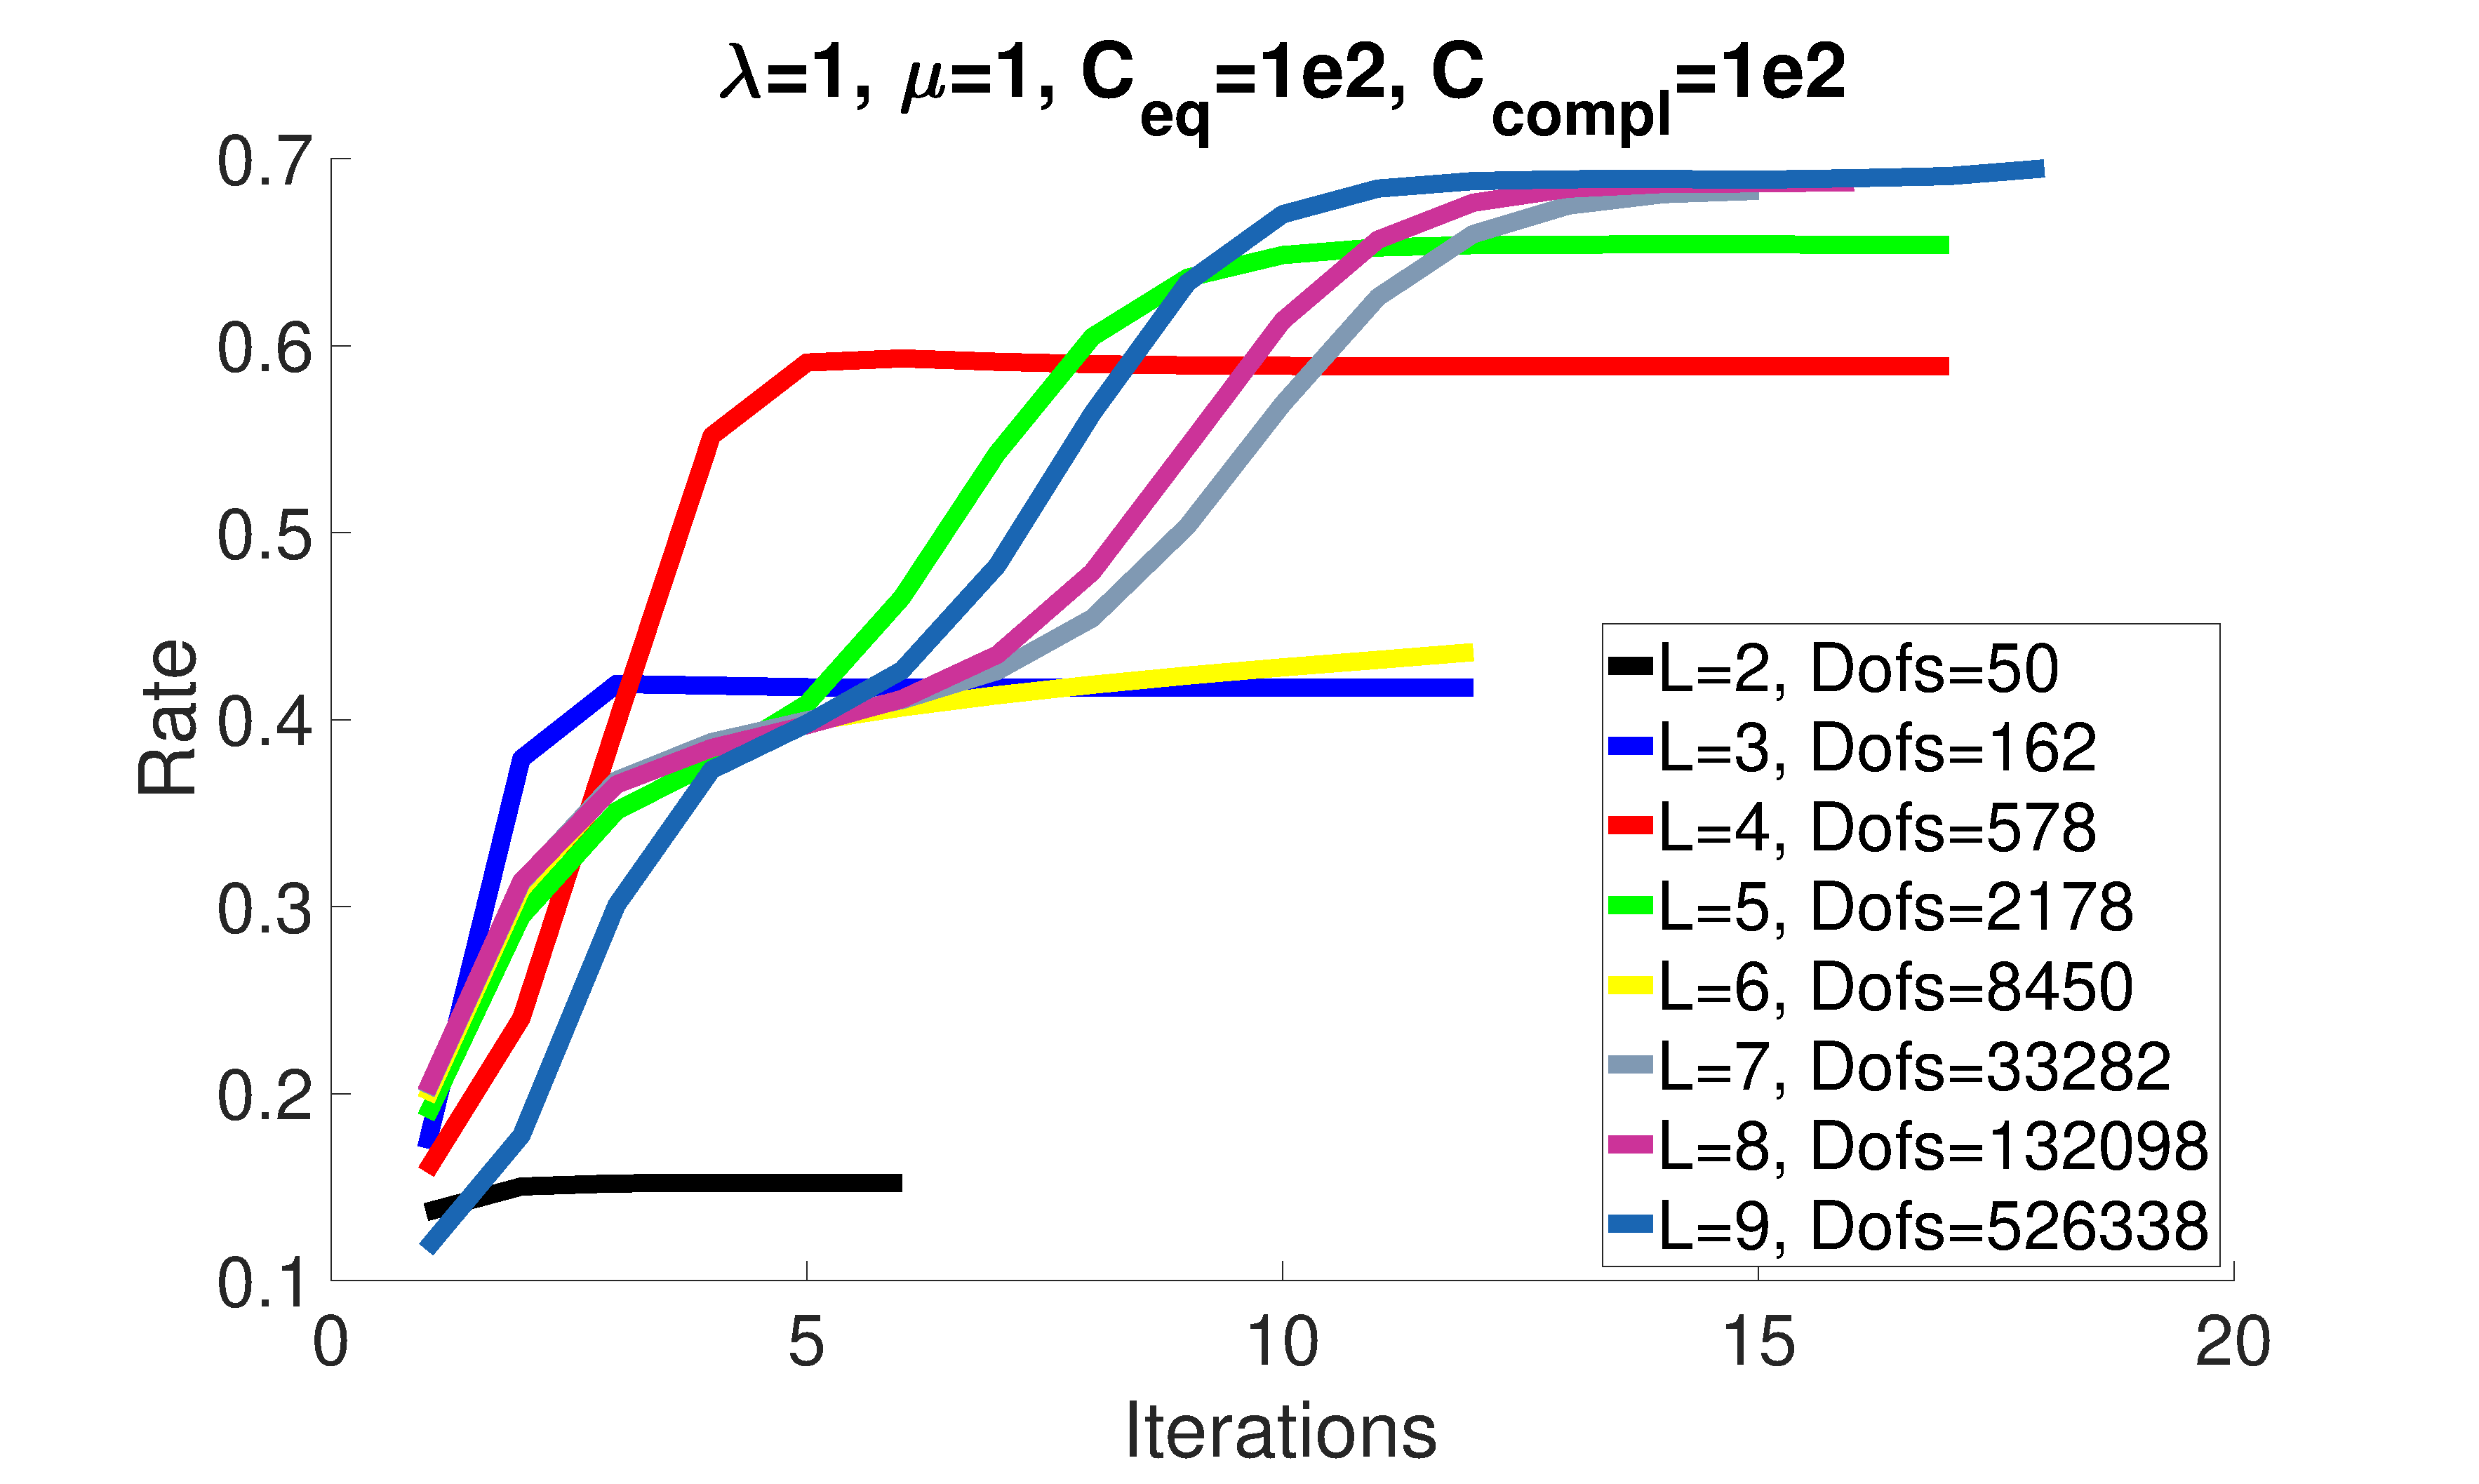
\includegraphics[scale=0.08]{img/SquareRateCompressible.eps}
	\caption{Square mesh. Compressible material.}
	\label{ResidualRateSquare}
	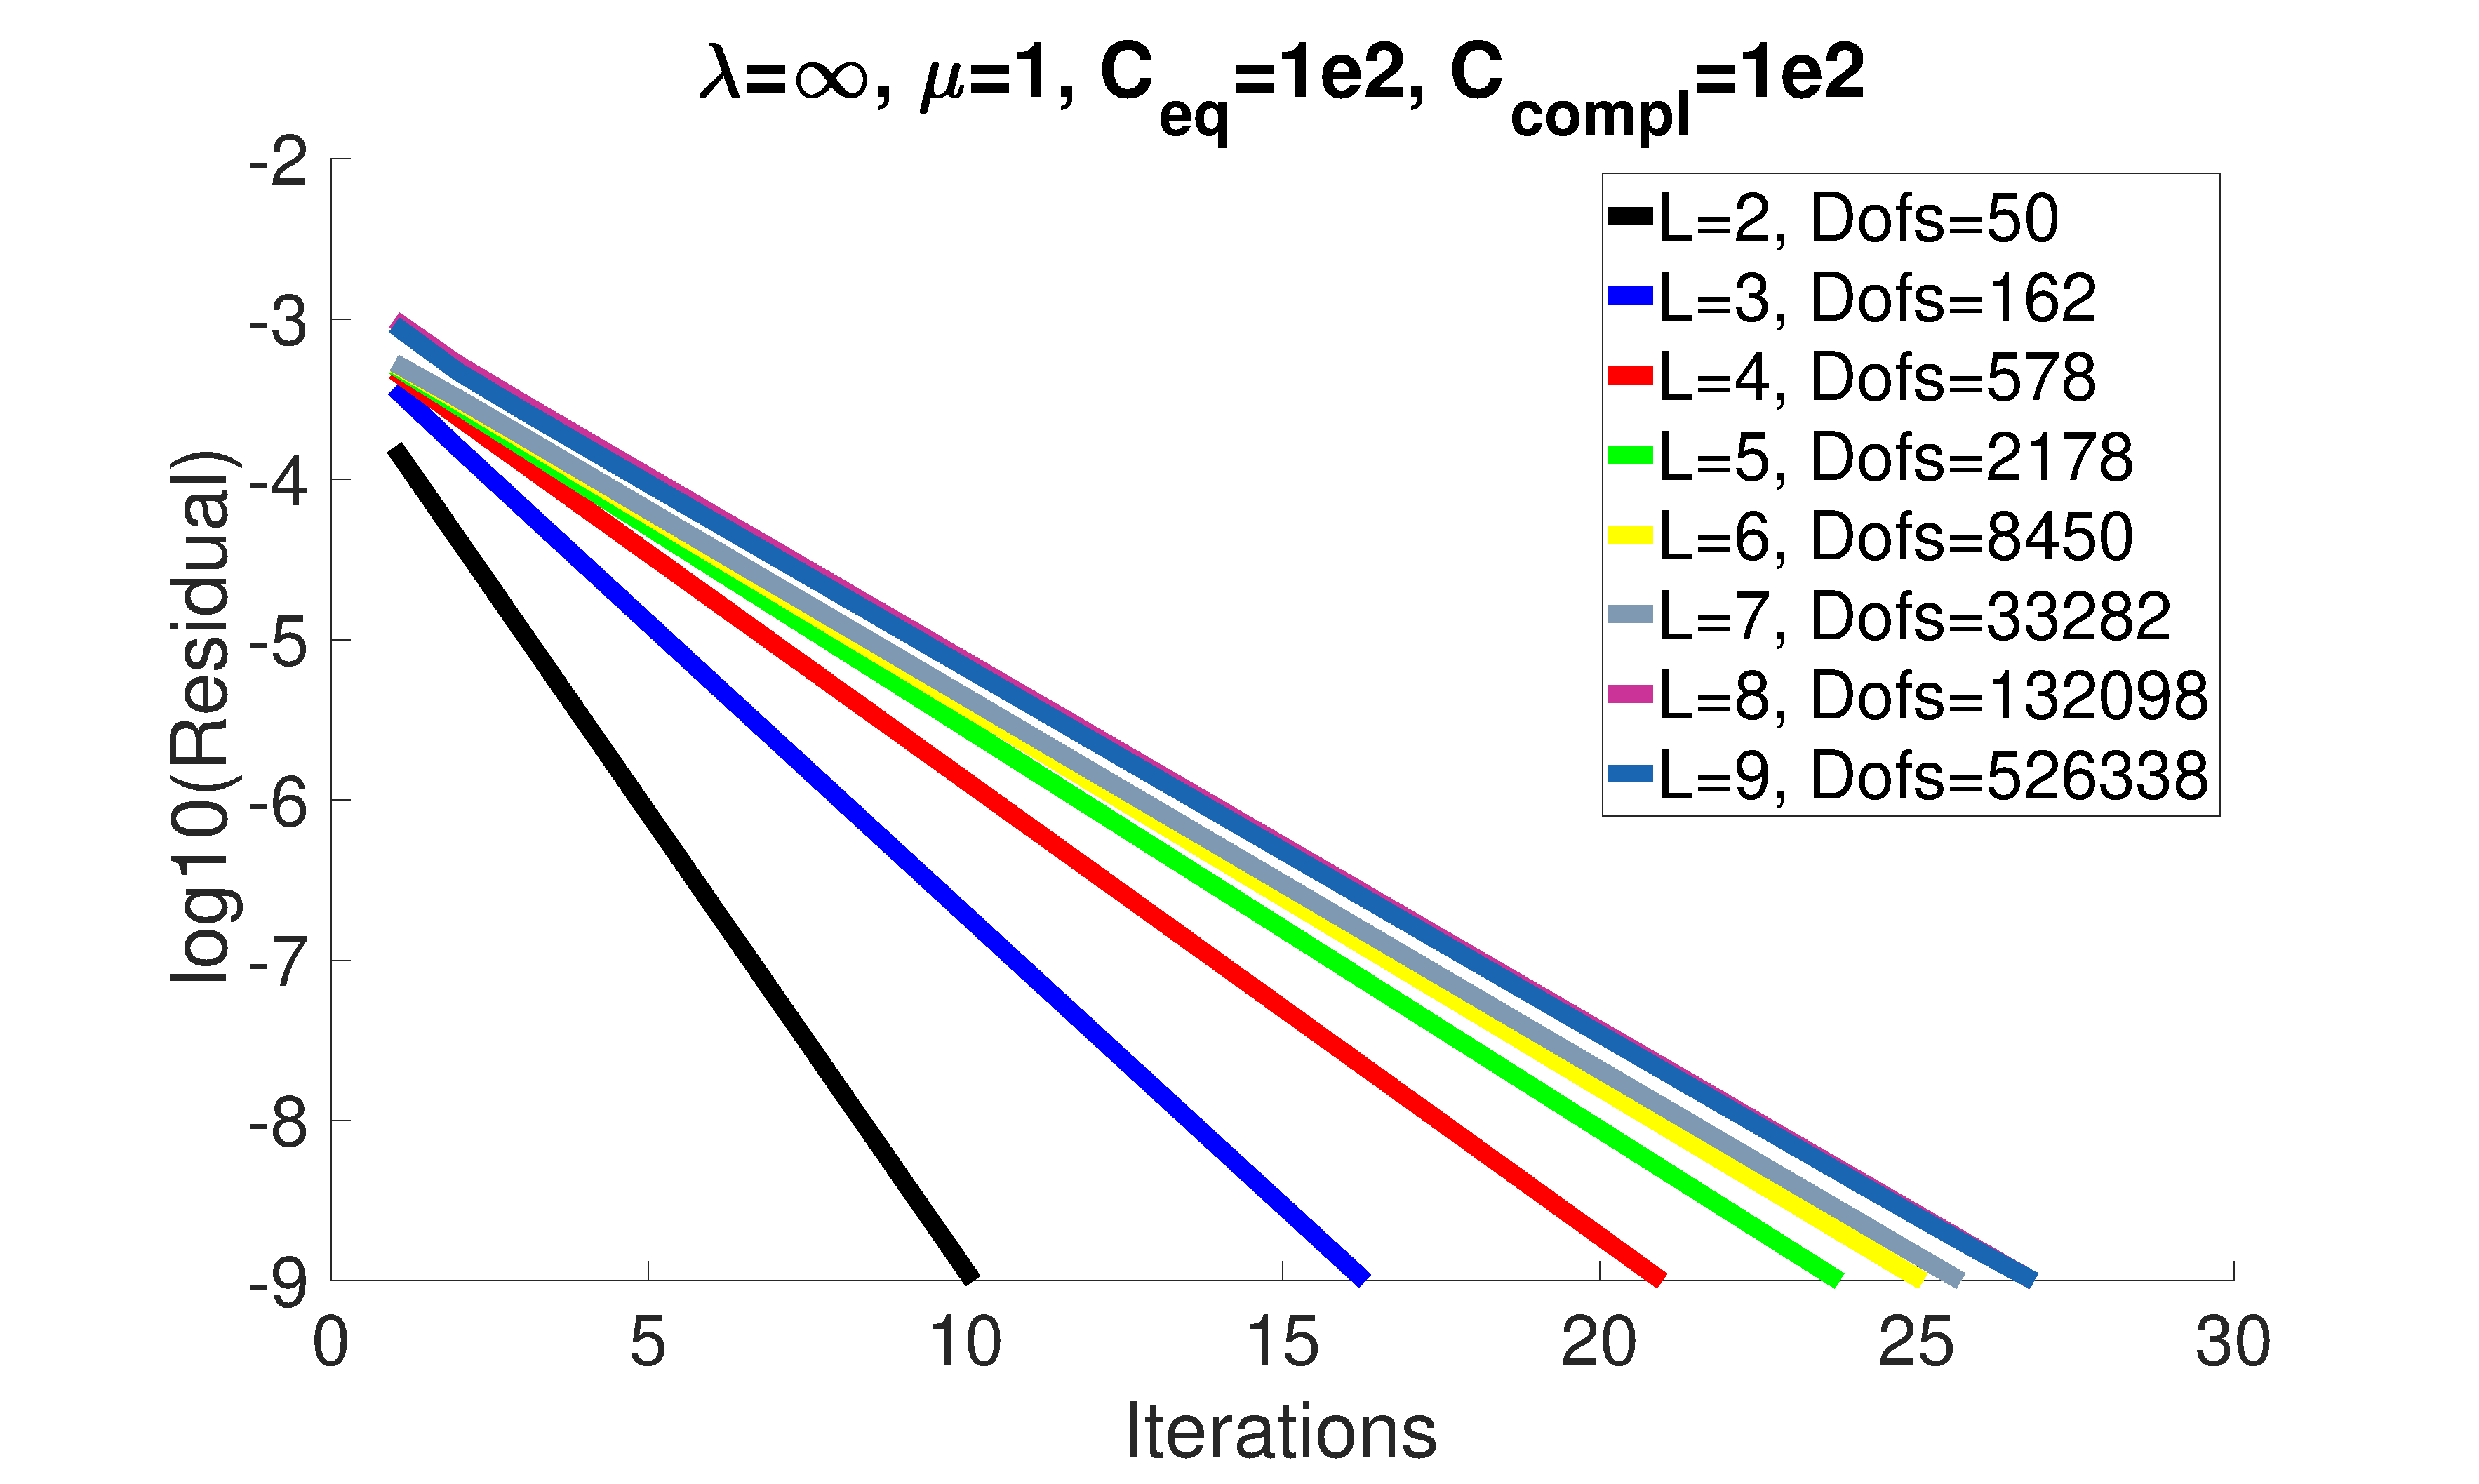
\includegraphics[scale=0.08]{img/SquareResidualIncompressible.eps}
	\quad
		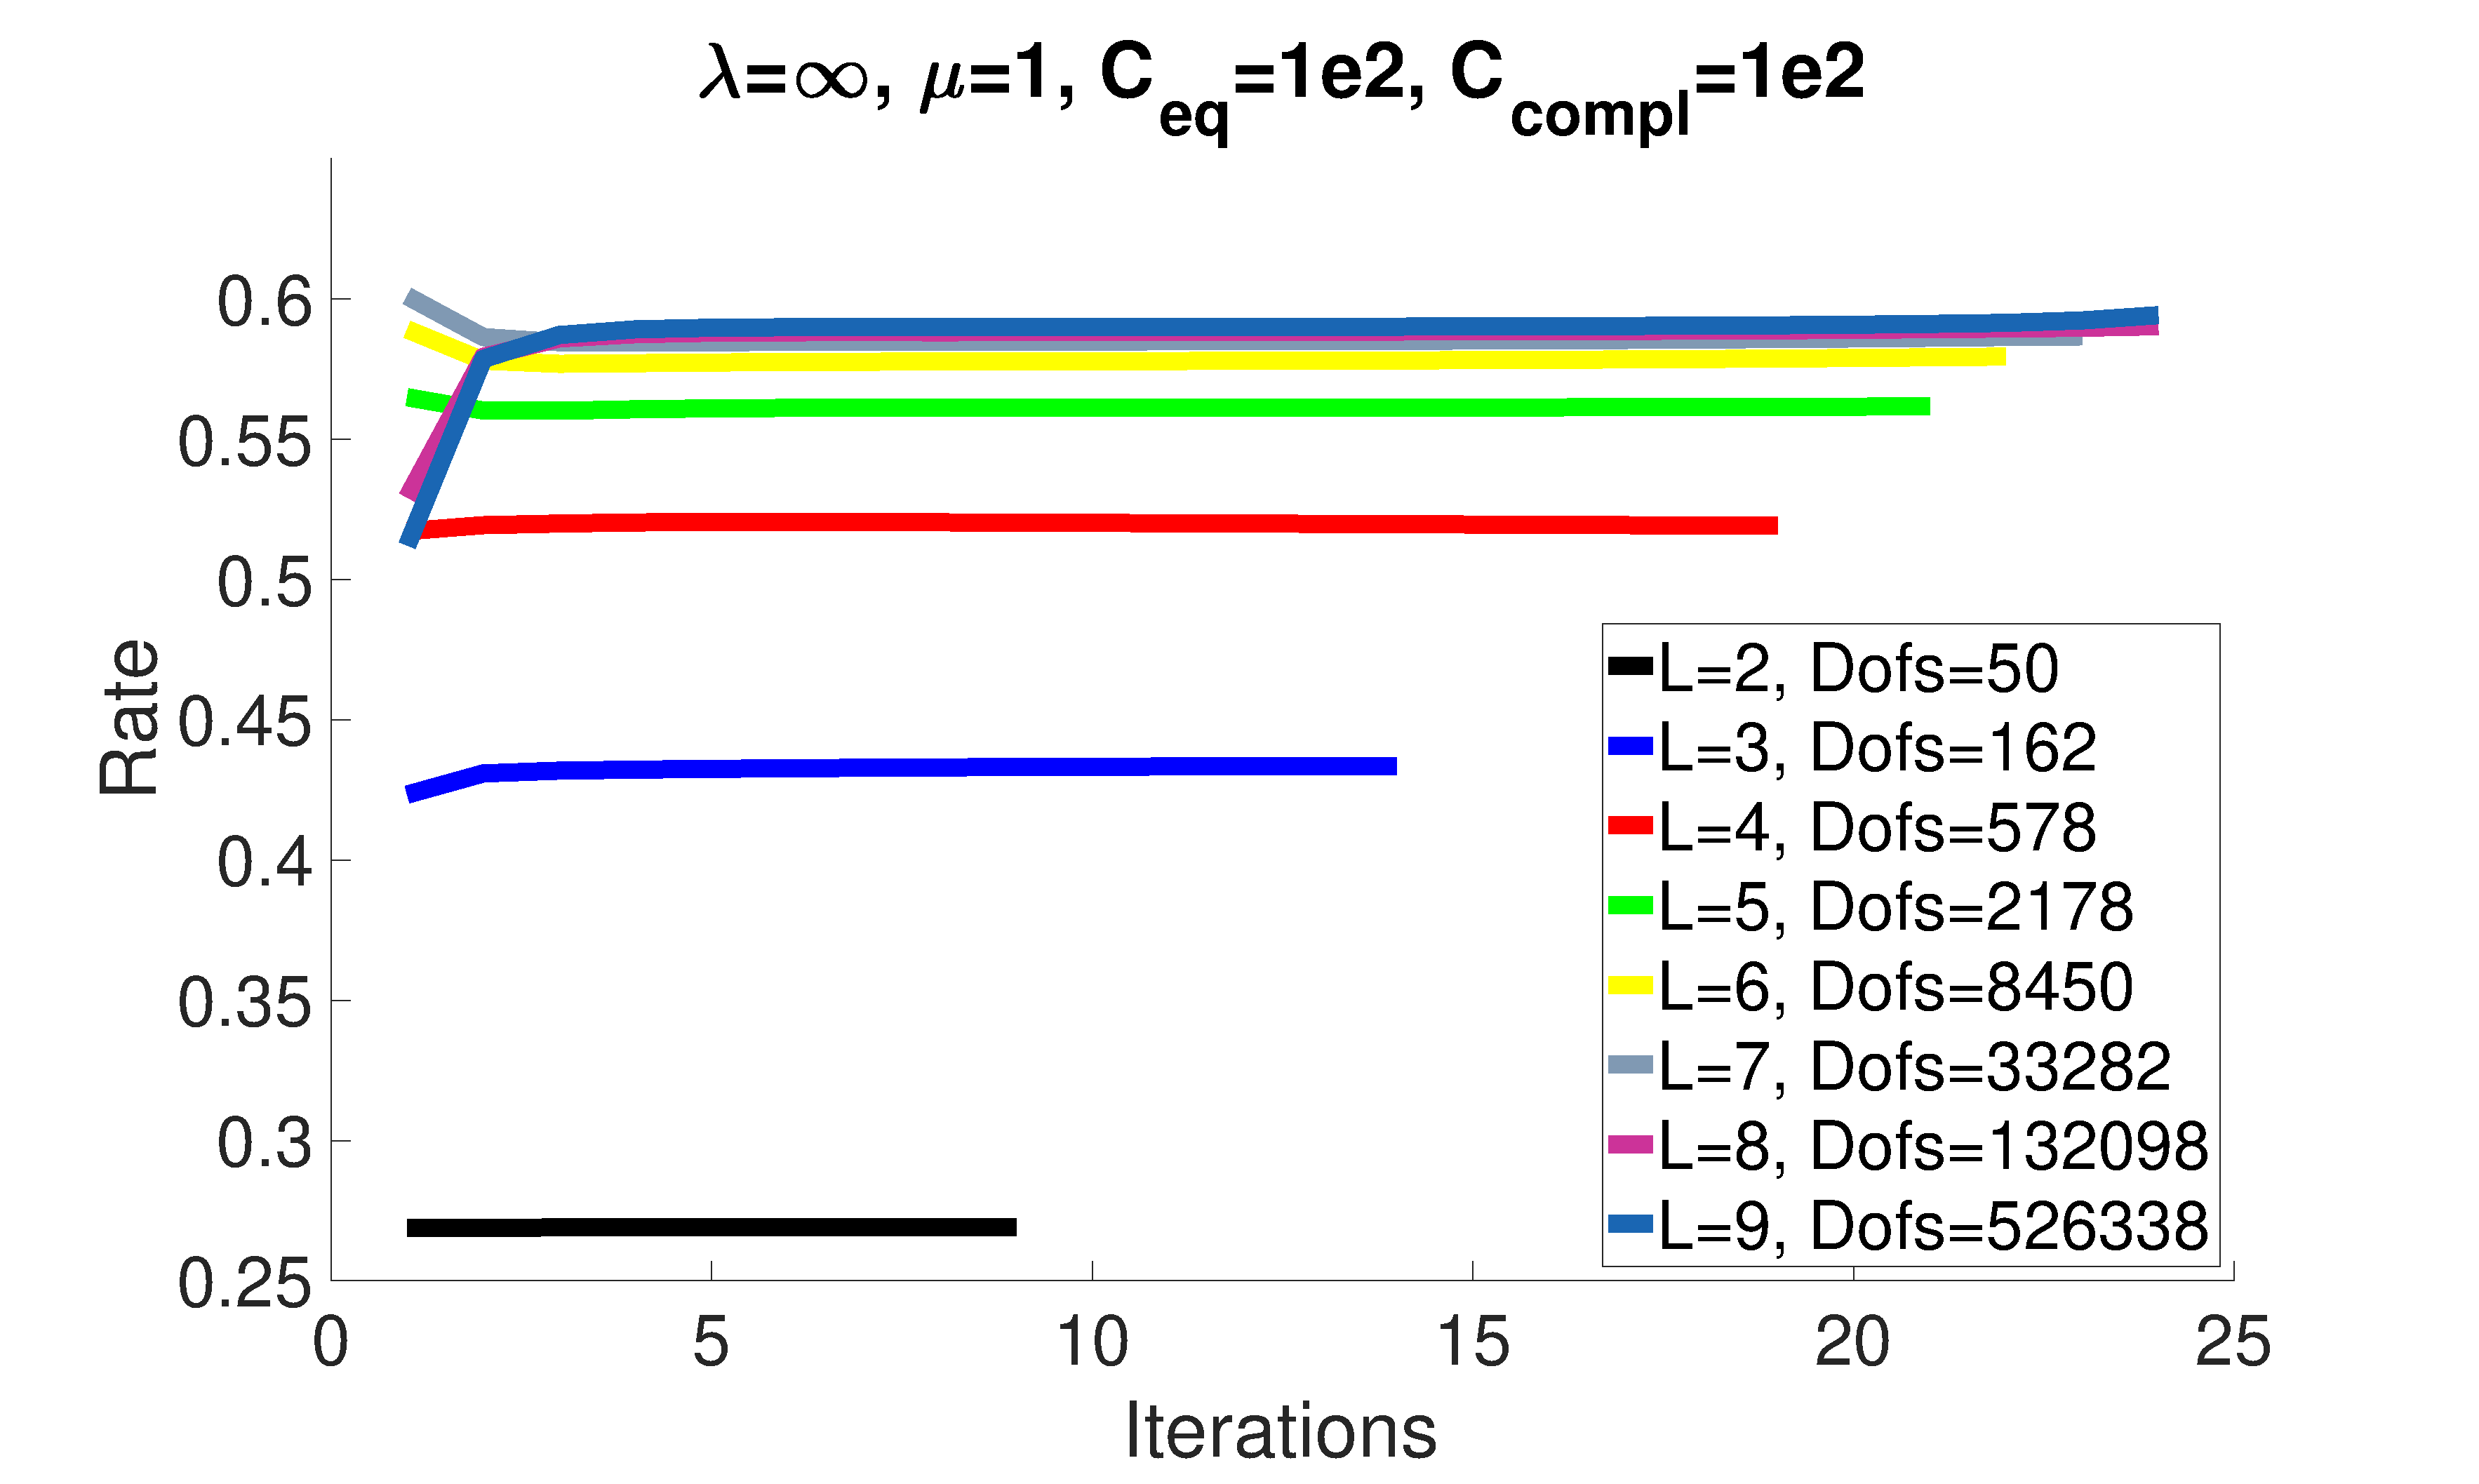
\includegraphics[scale=0.08]{img/SquareRateIncompressible.eps}
	\caption{Square mesh. Incompressible material.}
	\label{ResidualRateSquare}	
	\end{figure}
	$\bullet$ Purely linear problem: $h-$ and $J-$ independency
\end{frame}




%%%%%%%%%%%%%%%%%%%%%%%%%%%%%%%%%%%%%%%%%%
%%%%%%%%%%%               CONCLUSION          %%%%%%%%%%%%%%%
%%%%%%%%%%%%%%%%%%%%%%%%%%%%%%%%%%%%%%%%%%

\begin{frame}
\titlecolor{Conclusions}
\begin{itemize}
\item Monotone multilevel for FOSLS linear elastic contact 
${}$\\${}$\\
\item Limite case: $h$-- and $J$-- independency
${}$\\${}$\\
\item Similar behaviour of compressible and incompressible cases
\end{itemize}
\end{frame}


%%%%%%%%%%%%%%%%%%%%%%%%%%%%%%%%%%%%%%%%%%
%%%%%%%%%%%               THANK YOU          %%%%%%%%%%%%%%%
%%%%%%%%%%%%%%%%%%%%%%%%%%%%%%%%%%%%%%%%%%


\begin{frame}
\centering
\huge
Thank you for your attention!
\end{frame}

\begin{frame}
\end{frame}
\begin{frame}
\end{frame}

%%%%%%%%%%%%%%%%%%%%%%%%%%%%%%%%%%%%%%%%%%
%%%%%%%%%%%       LIFESAVING SLIDES       %%%%%%%%%%%%%%%
%%%%%%%%%%%%%%%%%%%%%%%%%%%%%%%%%%%%%%%%%%
%%%%%%%%%%%%%%%%%%%%%%%%%%%%%%%%%%%%%%%

\begin{frame}
\titlecolor{Exact Monotone Multilevel}
Define:
\begin{itemize}
\item $\bbx_J^k=(\bu_J^k,\bsigma_J^k) \in K_J$  $k$-th iterate
\item $\bbx_{J,0}=\bbx_{J}^k$
\item $\bbx_{j,0}=\bbx_{j+1,N_{j+1}}$, for $j=J-1,...,1$
\end{itemize}
Compute a sequence of intermediate iterates $\bbx_{j,\nu} =\bbx_{j,\nu-1}+\bc_{j,\nu}$:
\begin{align*}
&\mathcal{J}%(\bbx_{j,\nu}+\bc_{j,\nu})
 \leq \mathcal{J}(\bbx_{j,\nu}+\by) 
\quad \forall \by \in K_{j,\nu}^{*}\qquad j=J,...,2, \quad \nu=1,...,N_j\\
& \mathcal{J}(\bbx_{2,N_2}+\bc_{1}) \leq \mathcal{J}(\bbx_{2,N_2}+\by) \quad \forall \by \in K_{1}^{*}  \qquad j=1
\end{align*}
with the \textbf{exact} local closed convex sets $K_{j,\nu}^*$ and $K_1^*$:
\begin{align*}
\begin{aligned}
&  K_{j,\nu}^{*}(\bbx_{j,\nu})=\left\lbrace
\by \in \text{span}\{\blambda_{j,\nu}\}: \quad \by +\bbx_{j,\nu} \in K_J
  \right\rbrace  \\
  &  K_{1}^{*}(\bbx_{2,N_2})=\left\lbrace
\by \in \text{span}\{\blambda_{1}\}: \quad \by +\bbx_{2,N_2} \in K_J
  \right\rbrace 
  \end{aligned}
\end{align*}
${}$\\
${}$\\
\tiny{
Ralf Kornhuber. Monotone multigrid methods for elliptic variational inequalities I. Numerische Mathematik, 69(2):167-184, 1994.}
${}$\\${}$\\
\tiny{
 Ralf Kornhuber and Rolf Krause. Adaptive multigrid methods for Signorini's problem in linear elasticity. Computing and Visualization in Science, 4(1):9-20, 2001.}
\end{frame}



%%%%%%%%%%%%%%%%%%%%%%%%%%%%%%%%%%%%%%%%%%
%%%%%%%%%%%                   SLIDE 8                %%%%%%%%%%%%%%%
%%%%%%%%%%%%%%%%%%%%%%%%%%%%%%%%%%%%%%%%%%
\begin{frame}
\frametitle{\textbf{Approximate Monotone Multilevel}}
Define:
\begin{itemize}
\item $\bc_{j,\nu}=(\tilde{\bu}_{j,\nu},\tilde{\bsigma}_{j,\nu})$ correction at level $j$, patch $\nu$
\item $ \bc_{J,0}= \bbx_J^k $, $ \bc_{j,0}= \textbf{0} $ for $j=J-1,...,1$
\item $ \bw_{j,\nu}= \sum_{\mu=0}^{\nu}  \bc_{j,\mu}$ 
\end{itemize}
Compute a sequence of intermediate corrections $\bc_{j,\nu} \in K_{j,\nu}(\bw_{j,\nu-1})$  and $  \bc_{1}  \in K_1 $:
\begin{align*}
& { \mathcal{J}( \bw_{j,\nu-1}+\bc_{j,\nu}) \leq \mathcal{J}( \bw_{j,\nu-1}+\by) \quad \forall \: \by \in K_{j,\nu}} && j=J,...,2, \: \: \nu=1,...,N_j\\
&
{
  \mathcal{J}( \bc_{1}) \leq \mathcal{J}( \by) \quad   \:   \qquad \qquad \qquad \qquad \:
  \forall \: \by  \in K_1} \qquad  &&j=1
\end{align*}
with the \textbf{coarse convex sets} $K_j$ and the \textbf{approximate} local closed convex sets $K_{j,\nu}$:
\begin{align*}
&{ K_{j,\nu}(\bw_{j,\nu-1})=\left\lbrace
\by \in \text{span}\{\lambda_{j,\nu}\}: \: \by +\bw_{j,\nu-1} \in K_j
  \right\rbrace}\\
 &{   K_1 \subset K_2 \subset ... \subset K_{J-1}\subset K_J}
  \end{align*}
\end{frame}

%%%%%%%%%%%%%%%%%%%%%%%%%%%%%%%%%%%%%%%%%%
%%%%%%%%%%%                   SLIDE 9                %%%%%%%%%%%%%%%
%%%%%%%%%%%%%%%%%%%%%%%%%%%%%%%%%%%%%%%%%%

\begin{frame}
\titlecolor{Coarse Convex Sets and Constraints}
\footnotesize
{ \textbf{Coarse Convex Sets:}}
\begin{align*}
  K_j&=\left\lbrace
  \bbx_j=(\bu_j, \bsigma_j) \in X_j: \: \bu_j|_{\Gamma_D}=\bu_D , \:  \bsigma_j|_{\Gamma_N}=\bt_N, \right. \\
   & \left.
    \qquad \qquad  
  \: \bu_j\cdot \bn_j|_{\Gamma_C}\leq g_{j,u_n}, \: \bn^T(\bsigma_j \bn)  \leq g_{j,\sigma_n}, \: \bt_j^T(\bsigma \bn_j) =0
  \right\rbrace  \qquad j=J\\
  K_j&=\left\lbrace
  \bbx_j=(\bu_j, \bsigma_j) \in X_j: \: \bu_j|_{\Gamma_D}=\textbf{0} , \:  \bsigma_j|_{\Gamma_N}=\textbf{0}, \right. \\
   & \left.
    \qquad \qquad  
  \: \bu_J\cdot \bn_j|_{\Gamma_C}\leq g_{j,u_n}, \: \bn^T(\bsigma_j \bn)  \leq g_{j,\sigma_n}, \: \bt_j^T(\bsigma \bn_j) =0
  \right\rbrace  \qquad j=J-1,...,1
\end{align*}
{ \textbf{Coarse Constraints:}}
\begin{itemize}
\item
$\tilde{\bu}_{j,\nu}$ and $\tilde{\bsigma}_{j,\nu}$ are the components of the correction $\bc_{j,\nu}$.
 \begin{align*}
{ g_{j,u_n}}&=
\begin{cases}
g & j=J \\
I_{j+1,u_n}^j \left( g_{j+1,u_n} - \sum_{\nu=1}^{N_{j+1}} \left[ \tilde{\bu}_{j+1,\nu} |_{\Gamma_C} \right]_n\right) & j=J-1,...,1
\end{cases}\\
{ g_{j,\sigma_n}}&=
\begin{cases}
0 & j=J \\
I_{j+1,\sigma_n}^j \left( g_{j+1,\sigma_n} - \sum_{\nu=1}^{N_{j+1}}  \left[ \tilde{\bsigma}_{j+1,\nu} |_{\Gamma_C}\right]_n \right) & j=J-1,...,1
\end{cases}
\end{align*}
\end{itemize}
{ \textbf{Non-Linear Projection Operators:}}\\
$   I_{j+1,u_n}^j $, $   I_{j+1,\sigma_n}^j $ chosen so that ${   K_1 \subset K_2 \subset ... \subset K_{J-1}\subset K_J}$.
\end{frame}


\begin{frame}
\frametitle{Normal displacement Non-Linear Projection}
\footnotesize
\begin{align*}
\begin{aligned}
& v_H(\nu_{H,1}) \leq v_h(\nu_{H,1})\\
&  v_H(\nu_{H,2}) \leq v_h(\nu_{H,2})\\
&  \frac{1}{2}( v_H(\nu_{H,1}) + v_H(\nu_{H,2})) \leq v_h(\nu_{h})
\end{aligned}
\qquad \qquad \forall \varepsilon_H \in \mathcal{E}_H \cap \Gamma_{C,H}
\end{align*}
It is easy to see that, on $e_H$, the following values satisfy the three conditions above:
\begin{align*}
&
a)\quad\begin{cases}
\tilde{v}_H({\nu_{H,1}})= \min( v_h(\nu_{H,1}),\max( v_h(\nu_{h}), 2 v_h(\nu_{h}) - v_h(\nu_{H,2})) )\\
\tilde{v}_H({\nu_{H,2}})=\min( v_h(\nu_{H,2}),\max( v_h(\nu_{h}), 2 v_h(\nu_{h})- v_h(\nu_{H,1}) ) )
\end{cases}
&& \forall \varepsilon_H \in \mathcal{E}_H \cap \Gamma_C\\
&
b)\quad
\begin{cases}
\tilde{v}_H({\nu_{H,1}})= \min( v_h(\nu_{H,1}), v_h(\nu_{h}) )\\
\tilde{v}_H({\nu_{H,2}})=\min( v_h(\nu_{H,2}),v_h(\nu_{h} ) )
\end{cases}
&& \forall \varepsilon_H \in \mathcal{E}_H \cap \Gamma_C \\
&
c)\quad
\begin{cases}
\tilde{v}_H({\nu_{H,1}})= \min( v_h(\nu_{H,1}),v_h(\nu_{h}),  v_h(\nu_{H,2}) )\\
\tilde{v}_H({\nu_{H,2}})= \min( v_h(\nu_{H,1}),v_h(\nu_{h}),  v_h(\nu_{H,2}) )
\end{cases}
&& \forall \varepsilon_H \in \mathcal{E}_H \cap \Gamma_C
\end{align*}
\end{frame}




\begin{frame}
\frametitle{Pressure Non-Linear Projection}
\footnotesize
\begin{align*}
s_H(\phi_H) \leq s_h(\phi_h) \quad \forall \phi_h \in P_{\phi_H}^{\phi_h}
\end{align*}
Thus:
\begin{align*}
\displaystyle
&s_H=I_{h,\sigma_n}^H s_h= \sum_{\phi_{H_i} \in T_H} \left[ \lambda_{\Sigma_H,H_i}\right]_n \:s_H(\phi_{H_i})
\qquad \text{with} \qquad
 s_H(\phi_{H_i})= \min_{\phi_{h} \in P_{\phi_{H_i}}^{\phi_{h}}} s_h(\phi_h)
\end{align*}
\end{frame}


\begin{frame}
\frametitle{Truncated Basis}
\footnotesize
\begin{align*}
\label{truncatedbasis}
&
\left[\tilde{\blambda}_{U_j,\nu} \right]_i=
\begin{cases}
\left[\blambda_{U_j,\nu}\right]_i  & \nu \in \mathcal{N}_j \setminus  \mathcal{N}_{j}^{\bullet}, \: {i=n, t}   \\
0  & \nu \in   \mathcal{N}_{j}^{\bullet},\qquad \: {i=n}   \\
\left[\blambda_{U_j,\nu}\right]_i  & \nu \in\mathcal{N}_{j}^{\bullet}  , \qquad \: {i=t}   
\end{cases}
\\
&\left[\tilde{\blambda}_{\Sigma_j,\phi} \right]_i=
\begin{cases}
\left[\blambda_{\Sigma_j,\phi}\right]_i  & \phi \in \mathcal{F}_j \setminus  \mathcal{F}_{j}^{\bullet}, \: {i=n, t}   \\
0  & \phi \in   \mathcal{F}_{j}^{\bullet} \quad \quad\:\:\: {i=n}   \\
\left[\blambda_{\Sigma_j,\phi}\right]_i  & \phi \in\mathcal{F}_{j}^{\bullet}  , \qquad {i=t}   
\end{cases}
\end{align*}
\end{frame}





\end{document}  